\chapter{ Évaluation des méthodes de sur-segmentation}

\section{Introduction}
Nous devons l'introduction et la définition du concept de superpixel à Ren \textit{et al.} \cite{ren2003learning}. Petites régions homogènes et régulières, les superpixels forment une sur-segmentation de l'image. Un exemple où les contours des superpixels sont tracés en blanc est donné sur la figure \ref{fig:sp_exempleSp}.

L'utilisation des superpixels comme primitives visuelles présente de nombreux avantages. Notamment :
\begin{itemize}
\item les superpixels constituent des primitives visuelles bien moins nombreuses que les pixels, ce qui  permet de réduire considérablement les temps d'exécution de l'algorithme qui les manipule ;
\item les superpixels, parce qu'ils correspondent à des ensembles de pixels, fournissent une information plus riche (il est notamment possible de décrire leur texture ou leur géométrie).
\end{itemize}

Durant les vingt dernières années, les superpixels ont été intégrés de manière fructueuse au sein de \modif{nombreux travaux, tels} que la méthode de segmentation sémantique  proposée par Gould \textit{et al.} \cite{gould2008multi} ou, plus récemment, \modif{celle} de Zang \textit{et al.} \cite{zhang2016detecting} sur la catégorisation fine d'images. Ces succès ne doivent cependant pas masquer les difficultés inhérentes à la sur-segmentation et qui se cristallisent autour de la recherche d'un compromis capable de satisfaire au mieux trois objectifs : 
\begin{itemize}
\item la production de superpixels ne chevauchant pas les contours de l'image ;
\item l'obtention d'un faible nombre de superpixels afin de compresser au maximum la représentation de l'image ;
\item l'obtention d'un faible temps de calcul, garantissant que le bénéfice à utiliser les superpixels à la place des pixels ne soit pas compensé par le temps nécessaire pour les produire. 
\end{itemize}

Or, ces trois propriétés se révèlent contradictoires. En effet, la production de superpixels peu nombreux \modif{--} donc regroupant un nombre plus important de pixels \modif{--} augmente le risque de commettre des erreurs. Réduire cette erreur requiert une complexification des algorithmes, qui se répercute alors sur les temps de \modif{calcul}. Ainsi, aujourd'hui encore,  la sur-segmentation demeure un  champ de recherche actif, où de nouvelles propositions sont faites régulièrement \cite{achanta2012slic,conrad2013contour,machairas2015waterpixels}. 

\begin{figure}[htb]
	\centering
			\includegraphics[width=0.65\textwidth]{images/sur-segmentation/exempleSp}
		 \caption{Exemple de sur-segmentation. Les contours des superpixels sont tracés en blanc.}
		 \label{fig:sp_exempleSp}
\end{figure}


\section{Quelques exemples pratiques d'utilisation des superpixels}
L'analyse des méthodes intégrant une étape de sur-segmentation nous semble un préliminaire indispensable pour déduire les propriétés qui doivent être satisfaites par un algorithme de sur-segmentation, afin que celui-ci puisse être utilisé de manière fructueuse. La profusion des travaux reposant sur une étape sur-segmentation interdit toutefois de les décrire de manière exhaustive. Aussi avons-nous choisi trois applications représentatives.

\subsection{Segmentation sémantique}
Publiée en 2008, la méthode de segmentation sémantique de Gould \textit{et al.} \cite{gould2008multi} constitue une étape notable,  tant pour le domaine de la segmentation sémantique que pour celui de la sur-segmentation. Afin d'identifier et de localiser les différents objets composant une photographie, Gould \textit{et al.} proposent une méthode capable, à partir d'un ensemble de données d'apprentissage, de déduire les caractéristiques visuelles d'une catégorie d'objet ainsi que ses relations spatiales avec d'autres types d'objets. Ainsi, la probabilité qu'un ensemble de pixels appartienne à la classe \emph{vache} dépend à la fois de sa couleur, de sa texture et de la présence de pixels voisins attribués à des classes considérées comme probables, telle que \emph{l'herbe}. 

Les motivations évoquées pour justifier l'utilisation de superpixels à la place des pixels rejoignent celles \modif{avancées} par Ren \textit{et al.} \cite{ren2003learning} : la réduction du nombre de primitives manipulées, donc la diminution du temps de calcul global de l'application ainsi que l'utilisation de primitives visuelles contenant une information plus riche. Ainsi, chaque superpixel est décrit à la fois par sa couleur moyenne (\modif{espaces RGB et Lab}), sa texture (\modif{textons}) et sa géométrie. 

Les superpixels étant organisés en graphe, la probabilité pour un superpixel d'appartenir à chacune des classes dépend de ses caractéristiques visuelles propres ainsi que de la probabilité de ses voisins d'appartenir à la même classe ou à une classe fréquemment voisine. Or, contrairement aux pixels qui sont organisés en grille régulière, les superpixels forment un graphe sur lequel peu d'hypothèses simplificatrices peuvent être faites. En particulier\modif{,} la complexité du voisinage d'un superpixel, ou\modif{,} en d'autres termes\modif{,} son nombre de voisins, peut avoir un impact significatif sur le temps d'exécution. 

\subsection{Détection d'obstacle dans un environnement 3D}
Dans leur article \cite{petrovai2014obstacle}, Petrovai \textit{et al.} décrivent un système complet d’assistance à la conduite, capable de générer une représentation 3D de l'environnement dans lequel évolue le véhicule et de s'en servir pour détecter les obstacles présents sur la route, afin d'alerter le conducteur. Pour le rendre indépendant du véhicule, ils utilisent une tablette équipée de deux caméras. Ainsi\modif{,} l'algorithme de détection d'obstacles que Petrovai \textit{et al.} \cite{petrovai2014obstacle} décrivent répond à la nécessité de produire des résultats en temps réel -- permettant au conducteur de réagir promptement -- avec des contraintes matérielles fortes, les tablettes actuelles disposant de capacités de mémoire et de calcul limitées par rapport à celles d'un ordinateur. 

L'environnement 3D est déduit à partir des deux images prises par la tablette, grâce à une méthode de stéréovision : en identifiant pour chaque pixel de l'image de gauche son correspondant dans l'image de droite, la profondeur du point 3D correspondant à ces deux pixels est déduite. Pour des raisons d'efficacité, \modif{seules} quelques correspondances peuvent être identifiées entre les pixels des deux images, par comparaison de leurs caractéristiques. Elles permettent une représentation 3D partielle, qui sera ensuite étendue sur la base de la sur-segmentation en superpixels. Petrovai \textit{et al.} commencent par fusionner ces superpixels  en fonction de leurs similarités en termes de couleur. Puis ils utilisent l'information 3D obtenue à l'étape précédente ainsi qu'une analyse de la géométrie et du niveau de gris moyen des superpixels pour identifier la route et les obstacles, puis pour calculer leur distance par rapport au véhicule. 

Dans le cadre des travaux de Petrovai \textit{et al.}, l'utilisation d'une méthode de sur-segmentation est clairement motivée par la volonté de produire une application finale aussi rapide que possible. Afin d'éviter que des erreurs ne soient commises au moment de la sur-segmentation et propagées, voire amplifiées lors des étapes suivantes, l'algorithme de sur-segmentation est paramétré pour produire des superpixels dont l'aire avoisine les $170$ pixels. 

\subsection{Classification fine d'images}
La classification fine d'images consiste à identifier, à partir d'une photographie, la présence d'objets appartenant à une même catégorie et présentant d'importantes similarités visuelles et sémantiques. Elle trouve de nombreuses applications en biologie,  par exemple pour identifier plusieurs espèces d'oiseaux, ainsi qu'en agronomie,  pour distinguer des plantes malades de celles en bonne santé.  Une part conséquente des travaux de recherche dans ce domaine consiste à proposer des descripteurs capables de \modif{différencier} chaque objet et ce, quel que soit le domaine de classification (champignons, marques de voitures, etc.). Comme les bases de données d'apprentissage peuvent, selon les domaines, contenir un nombre restreint de spécimens, des méthodes reposant sur une étape lourde d'apprentissage à partir d'un ensemble de données de référence \modif{composé} de plusieurs centaines d'images ne sont pas toujours envisageables. 

La méthode de Zhang \textit{et al.} \cite{zhang2016detecting} repose sur l'utilisation de primitives visuelles correspondant à de petits graphes qu'ils nomment \emph{graphlets}. Chaque sommet de ces graphlets correspond à un superpixel, donc un ensemble de pixels. Chaque paire de sommets ayant des pixels \modif{adjacents est} associée par une arête. Les graphlets sont ensuite caractérisés par leurs histogrammes de couleur en neuf dimensions \cite{stricker1995similarity}, leurs histogrammes de gradients orientés \cite{dalal2005histograms} et leurs structures\footnote{Par structure, nous entendons la manière dont \modif{ces} sommets sont connectés entre eux.}.  Pour des raisons de complexité algorithmique, il est souhaitable que les graphlets ne soient composés que d'un petit nombre de sommets. Zhang \textit{et al.} utilisent l'algorithme SLIC \cite{zhang2014probabilistic} proposé par Achanta \textit{et al.} \modif{\cite{achanta2012slic} pour} produire les superpixels. Trois niveaux de sur-segmentation sont produits, le nombre de superpixels, et donc leur aptitude à capter les détails fins, augmentant à chaque niveau.  Ainsi, les graphlets dont les sommets correspondent aux superpixels du premier niveau permettent de décrire les composantes les plus grandes de chaque objet (par exemple le corps d'un oiseau) tandis que ceux comprenant des superpixels du dernier niveau se focalisent sur des éléments plus petits (tels que le bec ou les pattes). Les graphlets comportent un nombre similaire de sommets, quel que soit le niveau de sur-segmentation.

Cette utilisation des superpixels est intéressante pour au moins trois raisons. Tout d'abord, l'un des intérêts  des superpixels réside dans leur faculté à suivre les bordures des objets bien plus finement que des patchs rectangulaires. Avec des séries de photos où le fond peut varier de manière significative, le fait d'utiliser un descripteur qui permette de se focaliser sur l'objet à identifier n'est sans doute pas anecdotique dans les excellents résultats obtenus par la méthode de Zhang \textit{et al.} Ensuite, chaque partie des objets est décrite en utilisant les relations de voisinage des superpixels. Enfin, le fait que trois niveaux de sur-segmentation soient utilisés découle de la difficulté actuelle pour un algorithme de sur-segmentation d'adapter l'aire des superpixels au niveau de détail. 

En effet, pour capter les détails les plus fins, de petits superpixels sont nécessaires. Comme la majorité des méthodes de sur-segmentation produisent des superpixels de taille \modif{quasi uniforme}, l'ensemble de l'image sera découpé en de nombreux superpixels. Au niveau des composantes plus grandes, ce nombre important de superpixels se traduit par des graphlets comprenant de nombreux nœuds, ce qui augmente significativement la complexité des traitements ultérieurs. 

\section{Évaluation d'un algorithme de sur-segmentation}
\subsection{Propriétés à évaluer}

De l'étude des trois applications précédentes, cinq propriétés permettant d'évaluer la qualité d'une sur-segmentation peuvent être énoncées. 
\begin{prop}[validité]
\label{prop1}
une sur-segmentation est considérée comme valide si elle constitue une partition de l'image en sous-ensembles connexes.
\end{prop}

\begin{prop}[adhérence aux contours]
\label{prop2}
un superpixel ne doit pas recouvrir différents objets de l'image.
\end{prop}

\begin{prop}[concision]
\label{prop3}
un algorithme de sur-segmentation doit produire aussi peu de superpixels que possible.
\end{prop}

\begin{prop}[simplicité]
\label{prop4}
le nombre de voisins d'un superpixel doit être aussi petit que possible.  
\end{prop}

\begin{prop}[rapidité]
\label{prop5}
un algorithme de sur-segmentation doit avoir un temps d'exécution aussi faible que possible.
\end{prop}

Pour que ces propriétés soient précises, il reste à définir ce que nous entendons par contour. À la différence d'autres travaux sur la sur-segmentation \cite{machairas2015waterpixels} nous ne pensons pas que ce terme doive se limiter aux contours en termes de couleur ou de  niveau de gris. Au contraire, il nous semble essentiel de prendre en compte la texture,  information dont le bénéfice est connu de longue date \cite{ozden2005image}.

La propriété \ref{prop1} indique que tout pixel doit être associé à un et un seul superpixel et qu'il existe, pour toute paire de pixels $(p_{i},p_{j})$ appartenant à un même superpixel $\mathbf{s}_{k}$, un chemin de pixels \modif{voisins} tous inclus dans $\mathbf{s}_{k}$, reliant $p_{i}$ à $p_{j}$. 

La propriété \ref{prop2} correspond à la définition d'une sur-segmentation : les contours des superpixels incluent les contours des objets dans l'image, mais sont plus nombreux que ces derniers. 

La propriété \ref{prop3} est liée au fait que les superpixels permettent un traitement plus efficace de l'information visuelle contenue dans l'image : moins ils sont nombreux, plus les traitements qui leur sont appliqués sont rapides. 

La propriété \ref{prop4} s'explique par le fait que, contrairement aux pixels, les superpixels ne forment pas un graphe avec une structure régulière en grille, ce qui induit des calculs supplémentaires lorsque le voisinage est pris en compte. Il est donc souhaitable que le nombre moyen de voisins d'un superpixel ne soit pas trop élevé.  

La propriété \ref{prop5} se justifie par le fait que la sur-segmentation d'une image est, dans la majorité des cas, un traitement préalable réalisé dans le but d'abaisser les temps d'exécution d'une méthode. Or le temps nécessaire pour produire les superpixels ne doit pas être supérieur au gain de temps apporté par leur utilisation à la place des pixels. 


\subsection{Évaluations précédentes}
\label{subsec:evalSpStatOfTheArt}

La première évaluation des méthodes de sur-segmentation a été réalisée en 2012 par Achanta \textit{et al.} \cite{achanta2012slic}. Elle compare les méthodes de \modif{Ren \textit{et al.} \cite{ren2003learning}}, Felzenszwalb \textit{et al.} \cite{felzenszwalb2004efficient}, Vedaldi \textit{et al.} \cite{vedaldi2008quick}, \modif{Levinshtein \textit{et al.} \cite{levinshtein2009turbopixels}}, Veksler \textit{et al.} \cite{veksler2010superpixels} et Achanta \textit{et al.} \cite{achanta2012slic}. Les six méthodes sont testées sur les $100$ images de la base de donnée de Berkeley \cite{MartinFTM01}, BSD\footnote{\url{https://www2.eecs.berkeley.edu/Research/Projects/CS/vision/bsds/}}. L'évaluation d'Achanta \textit{et al.} se concentre sur les propriétés \ref{prop2}, \ref{prop3} et \ref{prop5}.  


Afin de quantifier l'adhérence aux contours d'une sur-segmentation (propriété \ref{prop2}), Achanta \textit{et al.} utilisent deux mesures  : le taux d'erreur de sous-segmentation (\modif{$\mathcal{F}_{ES}$}) et le taux de rappel sur les contours (\modif{$\mathcal{F}_{RC}$}).  L'une comme l'autre sont calculées par rapport à une segmentation de référence $R$ à laquelle est comparée la sur-segmentation obtenue. Soit $\mathbb{S}=\lbrace \mathbf{s}_{1},\cdots, \mathbf{s}_{N_{\mathbb{S}}} \rbrace$ l'ensemble des superpixels. Le calcul du taux d'erreur de sous-segmentation repose sur la recherche, pour chaque \modif{région} $r_{i}$ \modif{présente} dans $R$, de l'ensemble des superpixels nécessaires pour le recouvrir et sur le nombre de pixels de cet ensemble  qui débordent de l'objet. Il est défini par : \modif{
\begin{equation}
\label{eq:superpixels:UE}
\mathcal{F}_{ES}(\mathbb{S},R) = \frac{1}{N_{I}} \sum_{r_{i} \in R} \sum_{ \mathbf{s}_{j} \cap r_{i} \neq \emptyset } \min(|\mathbf{s}_{j} \cap r_{i}| ,| \mathbf{s}_{j} - r_{i} |)
\end{equation}}
avec $N_{I}$ le nombre de pixels de l'image.  Le résultat obtenu est compris entre $0$ et $1$, un score de $0$ correspondant à une sur-segmentation sans erreur. 

Le taux de rappel sur les contours permet de vérifier que les contours des objets présents dans $R$ se retrouvent dans $\mathbb{S}$.  Soit $C_{R}$ l'ensemble des points de \modif{contour de la segmentation} de référence et $C_{\mathbb{S}}$ l'ensemble des points de \modif{contour de} la sur-segmentation. Si nous faisons l'hypothèse que\modif{,} pour chaque pixel\modif{,} nous savons sans aucun doute s'il appartient ou non aux contours, nous pouvons évaluer la qualité d'une sur-segmentation en calculant la proportion de points de \modif{contour} dans la \modif{segmentation} de référence qui correspondent à des points de \modif{contour} dans la sur-segmentation  : 
\begin{equation}
\label{eq:superpixels:br}
\mathcal{F}_{RC}(\mathbb{S},R) =   \frac { | C_{\mathbb{S}}  \cap C_{R} | }{ | C_{R} |}\text{.}
\end{equation} 
Concrètement, même pour un être humain, il n'est pas toujours aisé de déterminer au pixel près la position des contours \modif{dans une image}. Achanta \textit{et al.} se donnent une marge de deux pixels. Le score obtenu est compris dans l’intervalle $[0,1]$, un score de $1$ indiquant que tous les contours de $R$ se retrouvent dans $\mathbb{S}$. 

En outre, Achanta \textit{et al.} réalisent une étude de la complexité de chaque méthode ainsi que de ses temps d’exécution (propriété \ref{prop5}). Les scores pour les mesures \modif{$\mathcal{F}_{ES}$ et $\mathcal{F}_{RC}$}, ainsi que les temps d'exécution sont mis en relation avec le nombre de superpixels produits par la méthode, ce qui permet d'identifier les algorithmes capables de satisfaire aux mieux les propriétés \ref{prop2} et \ref{prop5} sous la contrainte de la propriété \ref{prop3}. 

Trois ans plus tard, une seconde évaluation a été menée par Stutz \modif{\textit{et al.} \cite{stutz2015superpixel}}.  Leur première contribution consiste en l'évaluation de 7 méthodes supplémentaires : Liu \textit{et al.} \cite{liu2011entropy},  Zhang \textit{et al.} \cite{zhang2011superpixels}, Conrad \textit{et al.} \cite{conrad2013contour}, Van \textit{et al.} \cite{van2012seeds}, Tang \textit{et al.} \cite{tang2012topology}, Weikersdorfer \textit{et al.} \cite{weikersdorfer2012depth} et Papon \textit{et al.} \cite{papon2013voxel}. Leur seconde contribution réside dans l'utilisation d'une deuxième  \modif{base de données}, celle de l'université de New \modif{York \cite{silberman2012indoor}}, NYU\footnote{\url{http://cs.nyu.edu}}, qui comprend $400$ images. Comme les \modif{tailles} des photographies dans les deux bases de données ne sont pas identiques ($481 \times 321$ pixels pour BSD, $640 \times 480$ pixels pour NYU), Stutz \textit{et al.} proposent de modifier le seuil de tolérance de la mesure $\mathcal{F}_{RC}$ en autorisant tous les pixels à une distance de $\nombre{0,0075} \times diag$, $diag$ \modif{étant la} longueur de la diagonale de l'image.  

Dans l'évaluation d'Achanta \textit{et al.} \cite{achanta2012slic}, les méthodes de Felzenszwalb \textit{et al.} \cite{felzenszwalb2004efficient} et d'Achanta \textit{et al.} \cite{achanta2012slic} obtiennent les meilleurs scores. L'étude de Stutz \modif{\textit{et al.} \cite{stutz2015superpixel}} confirme ce résultat et révèle que les méthodes de Vedaldi \textit{et al.} \cite{vedaldi2008quick}, Conrad \textit{et al.} \cite{conrad2013contour} et  Liu \textit{et al.} \cite{liu2011entropy} obtiennent des scores similaires à ceux de Felzenszwalb \textit{et al.} \cite{felzenszwalb2004efficient} et d'Achanta \textit{et al.} \cite{achanta2012slic}. Sur la base de données BSD, les scores optimaux sont atteints avec des sur-segmentations comprenant un millier de superpixels. Pour les cinq méthodes précédemment citées, le taux d'erreur de sous-segmentation est inférieur ou égal à $\nombre{0,04}$ et le taux de rappel supérieur ou égal à $\nombre{0,99}$. Pour la base de données NYU,  il faut environ $1500$ superpixels à ces mêmes méthodes pour obtenir des scores similaires. Le taux d'erreur de sous-segmentation est inférieur ou égal à $\nombre{0,09}$ et le taux de rappel, là encore, est supérieur ou égal à $\nombre{0,99}$. Pour les deux bases de données, ces performances sont obtenues pour un temps d’exécution d'environ une seconde par image, sur un ordinateur équipé de processeur \emph{Intel Core i7-3770} $\nombre{3,4}$ GHz et d'une RAM de $16$ Go. 

\subsection{Nécessité d'une évaluation complémentaire}
Les résultats obtenus par les deux évaluations précédemment décrites \cite{achanta2012slic, stutz2015superpixel} pourraient nous amener à la conclusion que le problème de la sur-segmentation d'une image est actuellement résolu, cinq méthodes obtenant des scores proches d'un résultat parfait, avec par exemple un taux de rappel de $\nombre{0,99}$ alors que le score maximale atteignable est de $1$. Ces deux évaluations s'avèrent néanmoins critiquables sur deux points : 
\begin{itemize}
\item elles se cantonnent à l'utilisation de petites images de \modif{tailles} similaires (de l'ordre de quelques milliers de pixels) qui ne permettent pas d'apprécier le passage à l'échelle des algorithmes ;
\item  elles se limitent à évaluer l'aptitude des méthodes à produire une sur-segmentation comprenant peu d'erreurs pour un nombre de superpixels donné, sans s'intéresser à leur capacité à s'adapter à la complexité de l'image.
\end{itemize}  

Par \emph{passage à l'échelle} nous entendons le fait qu'un algorithme conserve ses performances quelle que soit la taille de l'image fournie en entrée. En particulier, si les scores évoqués dans la section précédente sont excellents, il est justifié de se demander si les algorithmes évalués conservent la même efficacité avec des images de plusieurs millions de pixels, bien plus proches de la taille des photographies obtenues aujourd'hui avec un appareil photo standard ou un smartphone.

La complexité de l'image désigne ici le nombre d'objets qu'elle contient, ainsi que leur niveau de détail. Nous donnons une illustration de ce concept sur la figure \ref{fig:sp_complexiteImage}, au travers de deux images correspondant à deux situations extrêmes.  Dans le premier cas (figure \ref{fig:sp_complexiteImage}a), nous nous attendons à ce qu'une sur-segmentation en assez peu de superpixels fournisse une compression raisonnable de l'image, où aucune information visuelle importante ne soit perdue. Dans le second cas (figure \ref{fig:sp_complexiteImage}b), la présence de nombreux petits objets, tels que les arbres, ainsi que le niveau de détail sur les bâtiments impose de produire des superpixels plus petits (donc plus nombreux), afin d'éviter que plusieurs superpixels ne chevauchent des objets différents. Cette notion de complexité globale d'une image peut aisément être étendue aux parties d'une même image, à l'instar de l'exemple donné par la figure \ref{fig:sp_complexiteImage}c. Ainsi, si la zone correspondant au ciel peut être sur-segmentée en un nombre restreint de grands superpixels, afin de capter les détails des bâtiments, il est nécessaire de produire de nombreux petits superpixels.
\begin{figure}[htb]
	\centering
	
	 \begin{subfigure}[B]{0.45\textwidth}	
			\includegraphics[width=\textwidth]{images/sur-segmentation/im_simple}
		  \caption{Image pouvant être considérée comme simple : un seul objet est visible. Ce dernier contient peu de détails.  Sa couleur comme celle du fond sont relativement uniforme.}
			\includegraphics[width=\textwidth]{images/sur-segmentation/im_complexe}
		 \caption{Image pouvant être considérée comme complexe : de nombreux objets sont visibles (les différents bâtiments, les arbres, etc.). En outre, les bâtiments comprennent de nombreux détails. Même pour un être humain, la tâche consistant à tracer le contour de chaque objet visible se révèle fastidieuse. }
	\end{subfigure}		
	~	
	\begin{subfigure}[T]{0.45\textwidth}	
			\includegraphics[width=\textwidth]{images/sur-segmentation/im_complexite_variable}
		 \caption{Image contenant des objets de complexité variable : tandis que le ciel correspond à une zone uniforme, les bâtiments contiennent de nombreux détails.  }
	\end{subfigure}
	\caption{Illustration de la notion de complexité à partir de trois photographies issues des données de référence de Berkeley \cite{MartinFTM01}.}
	\label{fig:sp_complexiteImage}
\end{figure}

Dans les trois cas de figure présentés, il est préférable de disposer d'un algorithme de sur-segmentation capable de faire varier automatiquement la taille des superpixels en fonction de la complexité de la zone dans laquelle ils se situent, sans qu'une modification \emph{ad hoc} de ses paramètres ne soit nécessaire. Nous désignons cette capacité d'un algorithme par le terme d'\emph{adaptabilité}. Par la suite, nous verrons que l'analyse de l'adaptabilité d'une méthode de sur-segmentation peut se faire par l'étude de l'évolution conjointe des propriétés \ref{prop2} et \ref{prop3}. 

\section{Proposition d'un nouveau protocole expérimental}
\label{sec:HSID-description-protocole-evaluation}
\subsection{Une nouvelle base de données : HSID}
L'ensemble de données de référence HSID, que   nous avons construit\modif{,} a été \modif{créé} à partir de 100 images issues de la base de données de Wikimedia Commons\footnote{\url{https://commons.wikimedia.org/wiki/Accueil}}. Nous avons sélectionné les photographies pour qu'elles présentent une large variété de difficultés : flou, bruit, ombre, faible contraste, reflet. Pour chacune de ces images, des contours ont été extraits par un être humain. 

Tout d'abord, pour chaque image, les objets qui seront séparés dans la segmentation de référence sont identifiés. Ces derniers sont choisis de manière à correspondre à des objets cohérents. Les objets sélectionnés correspondent aux objets principaux de la photographie ainsi qu'à des objets \modif{au} second plan, mais présentant des difficultés intéressantes.

Ensuite, une segmentation de référence est réalisée, sous forme d’aplats de couleurs, de manière à ce que deux objets voisins aient des couleurs différentes (figure \ref{fig:dataset_creation_step1}). Nous avons utilisé une tablette Intuos Pen ainsi que le logiciel de manipulation d'image Gimp. Enfin, les contours des segmentations sont extraits, un contour correspondant à un pixel ayant au moins un voisin (au sens du 8-voisinage)  de couleur différente (figure \ref{fig:dataset_creation_step2}). Cette dernière étape permet une vérification visuelle de la segmentation de référence créée. Si elle met en évidence des erreurs commises, celles-ci sont corrigées et une nouvelle vérification est effectuée.

\begin{figure}[htb]
	\centering
	 \begin{subfigure}[t]{0.3\textwidth}	
			\includegraphics[width=0.95\textwidth]{images/sur-segmentation/HSID/dataset_creation_step0}
		 \caption{Image d'origine}
		 \label{fig:dataset_creation_step0}
	\end{subfigure}		
	~
	 \begin{subfigure}[t]{0.3\textwidth}	
			\includegraphics[width=0.95\textwidth]{images/sur-segmentation/HSID/dataset_creation_step1}
		 \caption{Segmentation}
		 \label{fig:dataset_creation_step1}
	\end{subfigure}	
	~
	 \begin{subfigure}[t]{0.3\textwidth}	
			\includegraphics[width=0.95\textwidth]{images/sur-segmentation/HSID/dataset_creation_step2}
		 \caption{Extraction des contours}
		 \label{fig:dataset_creation_step2}
	\end{subfigure}	
	\label{fig:dataset-creation}
	\caption{Procédure suivie pour la création de HSID.}
\end{figure}


\subsection{Mesure de l'adhérence aux contours}

Les mesures d'adhérence aux contours tentent d'évaluer la capacité d'un algorithme de sur-segmentation à produire des superpixels ne chevauchant pas deux objets distincts. Traditionnellement, le taux d'erreur de sous-segmentation $\mathcal{F}_{ES}$ (équation \ref{eq:superpixels:UE}) et la mesure de rappel sur les contours $\mathcal{F}_{RC}$ (équation \ref{eq:superpixels:br}) sont utilisés. Les sections suivantes montrent cependant que HSID soulève des difficultés spécifiques, demandant de repenser ces deux mesures.

\subsubsection{HSID : un cas limite pour l'utilisation du taux d'erreur de sous-segmentation}
La figure \ref{fig:prob-ue} montre deux images de synthèse ($512\times1024$ pixels), correspondant à deux types d'images opposés : la première (figure \ref{fig:img-few-bdr}) contient un seul objet, de grande taille ; la seconde (figure \ref{fig:img-plenty-bdr}) contient de multiples petits objets. Le premier cas correspond à ce que nous obtenons avec une photographie de type portrait, se focalisant sur un seul objet d'intérêt. La seconde situation peut être assimilée à ce que nous obtenons avec une vue panoramique. 
\begin{figure}[htb]
	\centering
	
	 \begin{subfigure}[t]{0.45\textwidth}	
			\includegraphics[width=\textwidth]{images/sur-segmentation/UE/01-seg}
		 \caption{Image de type portrait et sur-segmentation sous la forme d'une grille régulière. $\mathcal{F}_{ES}(\mathbb{S},R)=\nombre{0,05}$.}
		 \label{fig:img-few-bdr}
	\end{subfigure}		
	~
	 \begin{subfigure}[t]{0.45\textwidth}	
			\includegraphics[width=\textwidth]{images/sur-segmentation/UE/10-seg}
		 \caption{Image de type panoramique et sur-segmentation sous la forme d'une grille régulière. $\mathcal{F}_{ES}(\mathbb{S},R)=\nombre{0,1}$.}
		 \label{fig:img-plenty-bdr}
	\end{subfigure}	
	\caption{Images de synthèse mettant en évidence les limites du taux d'erreur de sous-segmentation. Les zones grises correspondent au fond, les zones noires aux objets. Les contours des superpixels sont tracés en blanc. }
	\label{fig:prob-ue}
\end{figure}

Pour ces deux images\modif{,} nous avons produit une sur-segmentation en grille régulière, avec des cases carrées de $32\times32$ pixels. Comme le montre l'affichage des contours de cette sur-segmentation (figure \ref{fig:prob-ue}), dans les deux cas,  la sur-segmentation obtenue comporte de nombreuses erreurs, avec des superpixels dont les contours ne coïncident pas avec ceux des objets visibles. Nous sommes capables de ce diagnostic, car nous focalisons \modif{notre attention} sur les superpixels au niveau des contours des objets. En effet, les superpixels à l'intérieur des différents objets ne contiennent pas d'erreurs et il en serait de même, \modif{quelle que} soit leur forme. Or, ces derniers sont malgré tout pris en compte lors du calcul du taux d'erreur de sous-segmentation $\mathcal{F}_{ES}$, qu'ils contribuent à \modif{diminuer}. Ainsi dans le cas de l'image de la figure \ref{fig:img-few-bdr} où ces superpixels sont plus nombreux, le score $\mathcal{F}_{ES}$ bien meilleur : $\nombre{0,05}$ contre $\nombre{0,1}$ pour l'image de la figure \ref{fig:img-plenty-bdr}.

Les images des données de référence BSD et NYU correspondant essentiellement à des prises de vue panoramiques, le taux moyen d'erreur de sous-segmentation est un indicateur acceptable. Il n'en va pas de même pour HSID, qui comprend les deux situations extrêmes décrites ci-dessus, avec des segmentations de référence allant de deux à une dizaine d'objets. Dans ces conditions, le score moyen, médian, maximum ou minimum obtenu pour la mesure  $\mathcal{F}_{ES}$  ne permet de quantifier correctement l'adhérence aux contours. Nous avons donc choisi de ne pas utiliser la mesure  $\mathcal{F}_{ES}$ .


\subsubsection{Amélioration de la mesure d'adhérence aux contours}

Lors de la réalisation des segmentations de référence, nous avons constaté que, pour un certain nombre des images de HSID, il n'était pas possible de déterminer au pixel près où se situent les contours. C'est par exemple le cas lorsqu'un objet est flou \modif{ou en présence} de fourrure ou de cheveux qui comprennent une part de transparence. 
La grande variété des \modif{tailles} des images \modif{de HSID} rend inutilisable la mesure d'adhérence proposée par Achanta \textit{et al.} \cite{achanta2012slic}, $\mathcal{F}_{RC}$ (équation \ref{eq:superpixels:br})\modif{,} qui utilise un seuil de tolérance fixe, une erreur de deux pixels n'ayant pas du tout la même importance pour une image de $300 \times 400$ pixels que pour une image de $3000 \times 4000$ pixels. Quant à celle proposée par Stutz \textit{et al.} \cite{stutz2015superpixel}, elle s'avère inadaptée pour des images de grande taille, le seuil de tolérance s'élevant alors à une trentaine de pixels, ce qui dépasse largement l'erreur acceptable, y compris dans les pires cas. Ces raisons nous ont conduit à concevoir une nouvelle mesure d'adhérence aux contours, dont la définition s'appuie sur la théorie des sous-ensembles flous. 

Soit $R$  la segmentation de référence pour une image donnée et $\mathbb{S}$  la sur-segmentation obtenue pour cette image. \modif{L'ensemble $R = \lbrace r_{1}, \cdots, r_{N_{R}} \rbrace $} est une partition en $N_{R}$ composantes connexes et \modif{l'ensemble $\mathbb{S}  = \lbrace \mathbf{s}_{1}, \cdots, \mathbf{s}_{N_{\mathbb{S}}} \rbrace$} est une partition en $N_{\mathbb{S}}$ composantes connexes. Nous supposons que $N_{\mathbb{S}} > N_{R}$. 

Un pixel $p_{i}$ est un point de contour dans $\mathbb{S}$, si 
\modif{
\begin{equation*}
\exists p_{j} \in \nei(p_{i})\text{, } ( p_{i} \in \mathbf{s}_{n} \wedge p_{j} \notin \mathbf{s}_{n}) \text{.}
\end{equation*}}

De même, un pixel $p_{i}$ est un point de contour dans $R$, si 
\modif{
\begin{equation*}
\exists p_{j} \in \nei(p_{i})\text{, } ( p_{i} \in r_{n} \wedge p_{j} \notin r_{n}) \text{.}
\end{equation*}}

Soit $C_{R}$  l'ensemble des points de \modif{contour} de $R$ et $C_{\mathbb{S}}$ l'ensemble des points de \modif{contour} de $\mathbb{S}$. La proportion de points de contour de $R$ qui correspondent à des points de contour \modif{de} $\mathbb{S}$ est donnée par \modif{le taux de rappel des contours} $\mathcal{F}_{RC}$ (équation \ref{eq:superpixels:br}).

Comme les points de contour des superpixels qui se situent à l'intérieur d'un objet ne sont pas pris en compte, $\mathcal{F}_{RC}$ est similaire à une mesure d'omission qui serait calculée dans le cadre d'une classification des éléments de $C_{R}$ en deux classes :
\begin{itemize}
\item  \emph{l'élément appartient au contour d'un superpixel} ;
\item  \emph{l'élément n'appartient pas \modif{au} contour \modif{d'un des} superpixels}.
\end{itemize}

Soit \modif{le sous-ensemble} flou $C_{R \cap \mathbb{S}}^{*}$ défini à partir de $C_{R}$, avec la fonction d'appartenance  $f_{R \cap \mathbb{S}}$ qui donne pour un élément de $C_{R}$ son degré d'appartenance à un point de contour dans $C_{\mathbb{S}}$. La fonction $f_{R \cap \mathbb{S}}$  est définie de la manière suivante : 
\modif{\begin{equation}
f_{R \cap \mathbb{S}}(p_{i}) = \exp \left(- \frac{d(p_{i}-p_{i}')^{2}}{2\sigma^{2}} \right)
\end{equation}}
avec  :
\begin{itemize}
\item $d(p_{i}-p_{j})$ la distance entre $p_{i}$  et $p_{j}$  (par exemple la distance euclidienne) ;
\item \modif{$\sigma$ un paramètre pondérant l'influence de la distance entre $p_{i}$  et $p_{j}$, que nous avons fixé à $4$ après quelques tests empiriques} ;
\item \modif{$p_{i}'= \underset{p_{j} \in C_{\mathbb{S}}  } \argmin (d(p_{i}-p_{j}))$}. 
\end{itemize}

La fonction $f_{R \cap S}$ donne une valeur  dans l'intervalle $[0,1]$, la valeur $1$ correspondant au cas où un pixel dans $C_{R}$ coïncide parfaitement avec un pixel dans  $C_{\mathbb{S}}$. Il est \modif{ainsi} possible de définir une mesure floue d'adhérence au contour :
\modif{\begin{equation}
\label{eq:sp:FBR}
\mathcal{F}_{FRC}(\mathbb{S},R)  =  \frac{1}{|C_{R}|} \sum_{p \in C_{R}} f_{R \cap \mathbb{S}}(p)
\end{equation}}
C'est cette mesure que nous proposons d'utiliser pour évaluer l'adhérence aux contours d'une sur-segmentation. 
\section{Algorithmes évalués}

À ce jour, il existe une vingtaine de méthodes de sur-segmentation. Un quart d'entre elles sont initialement des algorithmes de segmentation \modif{\cite{comaniciu2002mean,felzenszwalb2004efficient, ren2003learning,vedaldi2008quick,vincent1991watersheds}} reconvertis grâce à une modification de leurs paramètres. Parmi les méthodes conçues  uniquement pour réaliser une tâche de sur-segmentation, une dizaine \modif{ \cite{achanta2012slic,conrad2013contour,levinshtein2009turbopixels,liu2011entropy,machairas2015waterpixels,papon2013voxel,tang2012topology,van2012seeds,veksler2010superpixels,weikersdorfer2012depth,zhang2011superpixels}} bénéficient d'une bonne notoriété, notamment parce qu'une implémentation ou un exécutable mis à disposition par leurs auteurs facilite leur \modif{réutilisation} au sein d'autres travaux. 

Nous nous sommes concentrés sur les cinq méthodes ayant obtenues les meilleurs scores lors de l'évaluation la plus récente, celle de Stutz \textit{et al.} \cite{stutz2015superpixel} : 
\begin{itemize}
\item la méthode Quick Shift \cite{vedaldi2008quick} (QS), qui consiste en une démarche similaire à celle de l'algorithme mean shift de Comaniciu \textit{et al.} \cite{comaniciu2002mean} ;
\item la méthode de Felzenszwalb \textit{et al.} \cite{felzenszwalb2004efficient} (FZ), qui repose sur un algorithme de coupure de graphe ;
\item la méthode de Liu \textit{et al.} \cite{liu2011entropy} (ERS\modif{, de l'anglais : \og \textit{Entropy Rate Superpixels} \fg}), qui groupe les pixels en ensembles homogènes et de même taille, par maximisation d'une fonction objectif ;
\item la méthode d'Achanta \textit{et al.} \cite{achanta2012slic} (SLIC), dont le traitement principal correspond à l’algorithme des $k$-moyennes et qui est sans doute l'algorithme de sur-segmentation le plus prisé ;
\item la méthode de \modif{Conrad \textit{et al.} \cite{conrad2013contour}} (CRS\modif{, de l'anglais :  \og \textit{Contour Relaxed Superpixels} \fg} ), dont l'originalité consiste à rechercher une sur-segmentation optimale à partir d'une sur-segmentation initiale, en ne modifiant que les pixels en bordure des superpixels. 
\end{itemize}

À ces cinq algorithmes, nous avons ajouté la méthode de Machairas \textit{et al.} \cite{machairas2015waterpixels} (WP\modif{, de l'anglais :  \og \textit{WaterPixels.}\fg}) et celle de Rubio \textit{et al.} \cite{rubio2016bass} (BASS\modif{, de l'anglais :  \og \textit{Boundary-Aware Superpixel Segmentation}\fg}), dont les publications sont concomitantes de celle de l'évaluation de Stutz \textit{et al.} \cite{stutz2015superpixel} et pour lesquelles aucune comparaison complète avec l'état de l'art n'existe. 

\subsection{\modif{Méthode de Vedaldi \textit{et al.} (QS)}}
La méthode QS, proposé par Vedaldi \textit{et al.} \cite{vedaldi2008quick} appartient à la catégorie des algorithmes de segmentation par recherche des modes. Soit $I$ une image. Vedaldi \textit{et al.}  \cite{vedaldi2008quick} décrivent les $N_{I}$ pixels qui la composent par leurs localisations et leurs couleurs. Ils obtiennent alors \modif{$X=\lbrace x_{1}, \cdots, x_{N_{I}} \rbrace$},  un  ensemble de $N_{I}$ vecteurs aléatoires à 5 dimensions. Les modes de la fonction de densité de probabilité associés à ces vecteurs aléatoires correspondent aux instances les plus fréquentes de ces vecteurs (donc aux maxima locaux de cette fonction).

La méthode QS permet de calculer efficacement ces modes et d'associer chaque pixel au mode dont les caractéristiques visuelles sont les plus proches des siennes. Les groupes de pixels ainsi obtenus forment une sur-segmentation de l'image. 

Soit $\phi$, une fonction fenêtre d'observation gaussienne, dont les pondérations sont données par :
\begin{equation}
w_{\phi}(n) = \exp \left( \dfrac{-n^{2}}{2\sigma^{2}} \right)
\end{equation} 
avec :
\begin{itemize}
\item $\dfrac{-(N_{\phi}-1)}{2} < n < \dfrac{(N_{\phi}-1)}{2}$, l'indice de la pondération ;
\item $N_{\phi}$ la taille de la fenêtre ; 
\item $\sigma$ l'écart type de la variable aléatoire considérée.  
\end{itemize}

La méthode QS \cite{vedaldi2008quick} repose sur une estimation de la densité de Parzen :
\modif{\begin{equation}
\mathcal{F}_{P}(x) = \dfrac{1}{N_{I}} \sum_{i=1}^{N_{I}}\phi(d(x - x_{i}))\text{, } x_{i} \in X\text{.}
\end{equation}}
 
À chaque itération de la méthode, chaque point correspondant à un vecteur $x_{i1}$ est déplacé vers $x_{i2}$, son plus proche voisin correspondant à une valeur plus élevée de la fonction de densité de Parzen :\modif{
\begin{equation}
i_{2} = \argmin_{i_{3} \in [1, N_{I}] } d(x_{i1},x_{i3})  \text{, } \mathcal{F}_{P}(x_{i1}) <  \mathcal{F}_{P}(x_{i3}) \text{.} 
\end{equation}}


\subsection{\modif{Méthode} de Felzenszwalb \textit{et al.} (FZ)}

L'algorithme de segmentation proposé par Felzenszwalb \textit{et al.} \cite{felzenszwalb2004efficient} groupe les pixels en régions, de manière à ce que les différences entres les pixels voisins et appartenant à des régions distinctes soient supérieures aux différences entre les pixels appartenant à une même région.

L'image $I$ est modélisée sous la forme d'un graphe \modif{$\mathcal{G}=\ <V,E>$} où $V=\lbrace v_{1},\cdots v_{N_{I}} \rbrace$ est un ensemble de $N_{I}$ sommets correspondant aux pixels de $I$ et $E$ un ensemble d'arêtes pondérées reliant les sommets $v_{i}$ et $v_{j}$ qui correspondent à des pixels voisins. Les régions sont formées en retirant un certain nombre d'arêtes satisfaisant un prédicat, de manière à obtenir une partition de $\mathcal{G}$ en composantes connexes correspondant à des ensembles de pixels homogènes. 


Soit $e_{i,j}$, l'arête reliant les sommets $v_{i}$ et $v_{j}$. La pondération $w_{i,j}$ associée à  $e_{i,j}$ est une mesure de la \modif{dissemblance} entre les pixels $i$ et $j$. Felzenzswalb \textit{et al.} proposent d'utiliser la valeur absolue de la différence entre les niveaux de gris des deux pixels. 


Soit $\mathbf{s}_{i}$ une composante connexe du graphe $\mathcal{G}$ et $E_{i} \subset E$ l'ensemble des arêtes reliant les sommets de  $\mathbf{s}_{i}$. La fonction 
\modif{\begin{equation}
\mathcal{F}_{Int}(\mathbf{s}_{i}) = \max_{e_{j,k} \in E_{i}}(e_{j,k})
\end{equation}}
correspond à une mesure du degré de \modif{dissemblance} entre les pixels composant $\mathbf{s}_{i}$.

Soit $E_{i,j}$ l'ensemble des arêtes reliant un sommet de la composante connexe $\mathbf{s}_{i}$ à un sommet de la composante connexe $\mathbf{s}_{j}$. La fonction 
\modif{\begin{equation}
\mathcal{F}_{Dif}(\mathbf{s}_{i},\mathbf{s}_{j}) = \min_{e_{k,l} \in E_{i,j}}(e_{k,l})
\end{equation}}
correspond à une mesure du degré de \modif{dissemblance} entre les deux composantes connexes $\mathbf{s}_{i}$ et $\mathbf{s}_{j}$. Si $E_{i,j} = \varnothing$, $\mathcal{F}_{Dif}(\mathbf{s}_{i},\mathbf{s}_{j})= \infty$. Le prédicat $\mathcal{F}_{P}$ défini par Felzenszwalb \textit{et al.} \cite{felzenszwalb2004efficient} est une fonction  binaire, qui renvoie \modif{vrai} si les deux composantes connexes doivent rester séparées, \modif{faux} si elles doivent être fusionnées : 
\begin{equation}
\mathcal{F}_{P}(\mathbf{s}_{i},\mathbf{s}_{j}) = \left\{
    \begin{array}{l}
       \text{vrai si } \mathcal{F}_{Dif}(\mathbf{s}_{i},\mathbf{s}_{j}) > \min\Big(\mathcal{F}_{Int}(\mathbf{s}_{i}) + \tau(\mathbf{s}_{i}) ,\mathcal{F}_{Int}(\mathbf{s}_{j}) + \tau(\mathbf{s}_{j})\Big)\text{,}\\
        \text{faux sinon, }
    \end{array}
    \right.
\end{equation}
avec  $\tau(\mathbf{s}_{i}) = \dfrac{\omega_{k}}{|\mathbf{s}_{i}|}$, où $\omega_{k}$ est un paramètre à déterminer lors de l'utilisation de l'algorithme et $|\mathbf{s}_{i}|$ correspond au nombre de sommets composant $\mathbf{s}_{i}$.

\subsection{\modif{Méthode} de Liu \textit{et al.} (ERS)}

L'algorithme ERS \cite{liu2011entropy}, reprend la représentation d'une image $I$ sous forme d'un graphe $\mathcal{G}$, semblable à celui \modif{défini pour la} méthode FZ. De manière similaire, Liu \textit{et al.} \cite{liu2011entropy} cherchent à retirer des arêtes de $E$, afin d'obtenir un ensemble de $N_{S}$ composantes connexes dont chacune correspond à un superpixel. Toutefois, contrairement aux travaux de Felzenszwalb \textit{et al.} \cite{felzenszwalb2004efficient} : 
\begin{itemize}
\item le nombre de composantes connexes est fixé par l'utilisateur et est respecté scrupuleusement par l'algorithme ;
\item les arêtes $e_{i,j} \in E$ sont pondérées par une mesure de similarité au lieu d'une mesure de \modif{dissemblance} ;
\item pour chaque sommet $v_{i}$, est ajoutée une arête $e_{i}$, qui boucle sur ce même sommet : \modif{lorsqu'une arête $e_{i,j}$ est supprimée, sa pondération est ajoutée sur les arêtes $e_{i}$ et $e_{j}$ ($e_{i} \leftarrow e_{i} + e_{i,j}$ et $e_{j} \leftarrow e_{j} + e_{i,j}$ ;}
\item la partition de $\mathcal{G}$ en composantes connexes est obtenue par maximisation d'une fonction objectif \modif{$\mathcal{F}_{ERS}$} : alors que l'algorithme FZ \cite{felzenszwalb2004efficient} repose sur une décision locale (l'arête $e_{i,j}$ \modif{doit-elle} être conservée ou non ?), ERS \cite{liu2011entropy} évalue l'impact global de la suppression de cette même arête.
\end{itemize}

Soit \modif{$\mathcal{G}^{*} =\ <V,E^{*}>$} le graphe résultat correspondant à la sur-segmentation. L'ensemble des arêtes $E^{*}$ correspond au sous-ensemble de $E$ pour lequel la fonction $\mathcal{F}_{ERS}$ atteint son maximum. Liu \textit{et al.} \cite{liu2011entropy} se donnent pour objectif d'obtenir des superpixels :
\begin{itemize}
\item dont les aires, en termes de nombre de pixels, sont similaires ;
\item qui ont une forte homogénéité interne en termes de couleur.  
\end{itemize}
La fonction \modif{de coût} \modif{est :
\begin{equation}
\mathcal{F}_{ERS}(\mathcal{G}') =  \mathcal{F}_{R}(\mathcal{G}') + \mathcal{F}_{E}(\mathcal{G}')
\end{equation}}
où les deux termes \modif{$\mathcal{F}_{R}$ et $\mathcal{F}_{E}$} s'assurent du respect des deux propriétés citées précédemment et $\mathcal{G}' =\ <V,E'> $ est un graphe intermédiaire, avec $E' \in E$.  

Soit $\mathbb{S}=\lbrace \mathbf{s}_{1}, \cdots, \mathbf{s}_{N_{\mathbb{S}}} \rbrace$ une partition de $\mathcal{G}$ en composantes connexes, après avoir supprimé une partie des arêtes de $E$. Nous notons $|\mathbf{s}_{i}|$ la cardinalité d'un ensemble $\mathbf{s}_{i}$. Liu \textit{et al.} \cite{liu2011entropy} définissent\modif{
\begin{equation}
\mathcal{F}_{R}(\mathcal{G}') = -N_{\mathbb{S}} -\sum_{i=1}^{N_{\mathbb{S}}} \dfrac{|\mathbf{s}_{i}|}{|V|}\log\Big( \dfrac{|\mathbf{s}_{i}|}{|V|} \Big) \text{.}
\end{equation}}
Cette fonction favorise non seulement des superpixels ayant la même aire, mais également les partitions des sommets de $V$ en exactement $N_{\mathbb{S}}$ composantes connexes.

Afin de mesurer l’homogénéité interne de chaque superpixel, Liu \textit{et al.} \cite{liu2011entropy} utilisent le taux d'entropie, une mesure qui permet de quantifier le  taux d'incertitude d'un processus aléatoire. Soit $\overline{E'}$ l'ensemble des arêtes supprimées. Les ensembles $E'$ et  $\overline{E'}$ forment une partition de $E$. 

\modif{Soient} $v_{i}$ et $v_{j}$ deux sommets.  Liu \textit{et al.} \cite{liu2011entropy} s'intéressent à la probabilité \modif{$P_{i,j}(\mathcal{G}',E') $} qu'un marcheur partant de $v_{i}$ arrive au sommet $v_{j}$. Cette probabilité est obtenue à partir de la mesure de similarité entre $v_{i}$ et $v_{j}$ :
\modif{\begin{equation}
P_{i,j}(\mathcal{G}',E') = \left\{
    \begin{array}{l l}
       \dfrac{w_{i,j}}{w_{i}} & \text{ si } i \neq j \text{ et } e_{i,j} \in E'\text{,}\\
       0	& \text{ si } i \neq j  \text{ et } e_{i,j} \in \overline{E'}\text{,}\\
       1- \dfrac{1}{w_{i}}  \sum\limits_{\substack{e_{i,k} \in  E'}} w_{i,k} 	& \text{ si } i = j\text{.}
    \end{array}
    \right.
\end{equation}}

\modif{Le graphe $\mathcal{G}'=\ <V,E'>$ peut être modélisé comme une marche aléatoire, sur laquelle il devient possible de calculer le taux d'entropie, mesurant l'homogénéité interne des superpixels} :
\modif{\begin{equation}
\mathcal{F}_{E}(\mathcal{G}',E')  = - \sum\limits_{\substack{v_{i} \in  V}} \left( \dfrac{w_{i}}{w_{V}} \sum\limits_{\substack{v_{j} \in  V}} P_{i,j}(\mathcal{G}',E') \log(P_{i,j}(\mathcal{G}',E'))\right)
\end{equation}}
avec \modif{$w_{V} = \sum\limits_{\substack{v_{i} \in  V}} w_{i}$.}

La recherche du graphe $\mathcal{G}^{*}$ permettant de maximiser $\mathcal{F}_{ERS}$ est réalisée par un algorithme glouton. \modif{En partant d'un ensemble $E'= \varnothing$, les arêtes de l'ensemble $E$ sont progressivement ajoutées à $E'$, en ajoutant à chaque itération l'arête permettant d'aboutir à l'augmentation la plus importante  de $\mathcal{F}_{ERS}$. L'algorithme s'arrête lorsqu'une partition de $V$ en exactement $N_{\mathbb{S}}$ composantes connexes est obtenue. Ces composantes connexes correspondent alors aux superpixels.}

\subsection{\modif{Méthode d'Achanta \textit{et al.} (SLIC)}}
\label{subsec:sp:slic}

La méthode \modif{SLIC} proposée par Achanta \textit{et al.} \cite{achanta2012slic}, correspond à une version modifiée de l'algorithme des $k$-moyennes. Elle est constituée de trois étapes : 
\begin{itemize}
\item l'initialisation, où une première sur-segmentation est donnée ;
\item le regroupement de pixels en ensembles, de manière à ce que chaque pixel soit rattaché à l'ensemble dont les caractéristiques visuelles sont les plus proches des siennes ;
\item le post-traitement s'assurant que les ensembles obtenus à l'étape précédente forment une partition en composantes connexes. 
\end{itemize}

Lors de l'étape d'initialisation, les pixels sont regroupés en superpixels correspondant à un découpage régulier de l'image sous la forme d'une grille. D'autres configurations peuvent également être envisagées, telles que des superpixels hexagonaux. 

La deuxième étape repose sur un processus itératif, répétant une dizaine de fois les actions suivantes :
\begin{enumerate}
\item  la couleur et la position \modif{moyennes} de ces $N_{\mathbb{S}}$ ensembles de pixels correspondant aux superpixels initiaux sont calculées ;
\item chaque pixel, décrit par sa couleur et sa localisation dans l'image, est assigné au superpixel dont il est le plus proche au sens d'une mesure de similarité ;
\item les caractéristiques des superpixels sont mises à jour.
\end{enumerate}

L'une des clés du succès de SLIC réside dans le fait que chaque pixel est comparé uniquement aux ensembles les plus proches, permettant à la méthode de produire une sur-segmentation avec une complexité quasi linéaire vis-à-vis du nombre de pixels dans l'image. 

Soit un superpixel $\mathbf{s}_{i}$ et $p_{j}$ un pixel. Nous notons $l_{i}$, $a_{i}$ et $b_{i}$ la couleur moyenne exprimée dans l'espace CIELab des pixels composant $\mathbf{s}_{i}$ ,  $x_{i}$ et $y_{i}$ les coordonnées du barycentre de $\mathbf{s}_{i}$, $l_{j}$, $a_{j}$ et $b_{j}$  la couleur de $p_{j}$, $x_{j}$ et $y_{j}$ ses coordonnées.  La similarité entre $\mathbf{s}_{i}$ et $p_{j}$ est évaluée par la fonction suivante :
\modif{\begin{equation}
\mathcal{F}_{SLIC}(\mathbf{s}_{i},p_{j}) = \sqrt{\mathcal{F}_{c}(\mathbf{s}_{i},p_{j} )^{2}  + \mathcal{F}_{p}(\mathbf{s}_{i},p_{j})^{2}  \Bigg( \dfrac{\omega_{C} N_{I}}{\sqrt{\omega_{\mathbb{S}}}}\Bigg) ^{2}}
\end{equation}}
avec :
\begin{itemize}
\item \modif{$\mathcal{F}_{c}(\mathbf{s}_{i},p_{j} )  =  \sqrt{(l_{i} - l_{j})^{2} +  (a_{i} - a_{j})^{2} + (b_{i} - b_{j})^{2}}$}, la distance euclidienne entre la couleur moyenne du superpixel et celle du pixel ;
\item  \modif{$\mathcal{F}_{p}(\mathbf{s}_{i},p_{j} )  =  \sqrt{(x_{i} - x_{j})^{2} +  (y_{i} - y_{j})^{2} }$}, la distance euclidienne entre le barycentre du superpixel et la position du pixel ;
\item $N_{I}$ le nombre de pixels de l'\modif{image};
\item \modif{$\omega_{C}$} un paramètre de compacité, pondérant l'influence de la position du pixel par rapport à sa couleur ;
\item $\omega_{N_{\mathbb{S}}}$ un paramètre indiquant le nombre de superpixels souhaités.
\end{itemize}

Soit $\mathbb{S}^{'}$ l'ensemble des superpixels ainsi obtenus. Les pixels étant regroupés aussi en fonction de leur couleur, il n'est pas garanti que  $\mathbb{S}^{'}$ forme une  partition de l'image en composantes connexes. Afin d'assurer le respect de la propriété \ref{prop1} (validité), les composantes connexes de $\mathbb{S}^{'}$  sont extraites. Celles dont le nombre de pixels est en dessous d'une taille minimale sont fusionnées avec une composante connexe voisine, donnant $\mathbb{S}$, la sur-segmentation finale.

\subsection{Méthode de Rubio \textit{et al.} (BASS)}

L'algorithme \modif{BASS de} Rubio \textit{et al.} \cite{rubio2016bass} est une version modifiée de SLIC, capable d'adapter le nombre de superpixels à la complexité locale de l'image : aux endroits contenant des objets de petite taille, de nombreux superpixels sont produits, tandis que les zones uniformes sont sur-segmentées en un nombre restreint de superpixels. Rubio \textit{et al.} introduisent deux changements :
\begin{itemize}
\item le premier, au niveau de l'étape d'initialisation, permet d'adapter le nombre de superpixels  de la sur-segmentation initiale; 
\item le second, au moment de l'évaluation de la similarité est l'ajout d'un terme capable de prendre en compte la présence d'un contour entre un pixel $p_{j}$ et le barycentre de l'ensemble $\mathbf{s}_{i}$.
\end{itemize}

Lors de l'étape d'initialisation, au moment de produire les superpixels initiaux suivant une grille, la méthode de Rubio \textit{et al.} commence par appliquer sur l'image le détecteur de \modif{contour de Doll\'{a}r \textit{et al.}} \cite{dollar2015fast} (évoqué dans la section \ref{subsec:sota:muller}). À partir du résultat de ce détecteur, une image binaire est produite où sont conservés, comme appartenant aux contours, tous les pixels pour lesquels la valeur du détecteur de contours \modif{se situe dans les} $70 \%$ des scores les plus élevés. 

Soit \modif{$\mathcal{F}_{C}$} la fonction qui, pour un ensemble de pixels, donne la portion de pixels appartenant à un contour. En particulier, \modif{$\mathcal{F}_{C}(I)$} correspond à la proportion de pixels appartenant à un contour dans l'image, et \modif{$\mathcal{F}_{C}(\mathbf{s}_{i})$} à celle des pixels appartenant à un contour au sein du superpixel $\mathbf{s}_{i}$. Les deux prédicats suivants permettent d'adapter le nombre de superpixels initiaux à la complexité de l'image :
\begin{itemize}
\item Si \modif{$\mathcal{F}_{C}(\mathbf{s}_{i}) > 3 \mathcal{F}_{C}(I)$}, alors le superpixel $\mathbf{s}_{i}$ appartient à une zone de l'image comprenant de nombreux détails : il est découpé en quatre nouveaux superpixels ;
\item Si  \modif{$\mathcal{F}_{C}(\mathbf{s}_{i}) < \mathcal{F}_{C}(I)$}, alors le superpixel $\mathbf{s}_{i}$ appartient à une zone de l'image relativement homogène et il est supprimé.
\end{itemize}
Afin de terminer l'étape d'initialisation, les composantes connexes correspondant aux  superpixels supprimés sont extraites : elles viennent s'ajouter à l'ensemble des superpixels initiaux, en plus des superpixels conservés et des superpixels nouvellement créés. 

La seconde contribution de Rubio \textit{et al.} consiste à proposer une nouvelle fonction permettant de calculer la similarité entre un superpixel $\mathbf{s}_{i}$ et un pixel $p_{j}$ :
\modif{\begin{equation}
\mathcal{F}_{BASS}(\mathbf{s}_{i},p_{j}) = \sqrt{\mathcal{F}_{c}(\mathbf{s}_{i},p_{j} ) + \omega_{p}\mathcal{F}_{p}(\mathbf{s}_{i},p_{j}) +\omega_{g} \mathcal{F}_{g}(\mathbf{s}_{i},p_{j})}
\end{equation}}
avec :
\begin{itemize}
\item \modif{$\mathcal{F}_{c}$ et $\mathcal{F}_{p}$} les deux fonctions décrites lors de la présentation de l'algorithme SLIC, dans la section précédente ;
\item \modif{$\mathcal{F}_{g}$} une fonction donnant la distance géodésique entre $p_{j}$ et $\mathbf{s}_{i}$ ;
\item $\omega_{p}$ et $\omega_{g}$, deux paramètres permettant de pondérer l'influence de chacun des termes.
\end{itemize}

Soit $p_{i} \in \mathbf{s}_{i}$ et $\zeta_{i,j}=(p_{i},\cdots,p_{j})$ un chemin discret le reliant à $p_{j}$. Soit $\Upsilon_{i,j}$ l'ensemble des chemins reliant $p_{j}$ à un pixel appartenant à $\mathbf{s}_{i}$. Rubio \textit{et al.} définissent :\modif{
\begin{equation}
\mathcal{F}_{g}(\mathbf{s}_{i}, p_{j}) = \min_{ \zeta_{i,j} \in \Upsilon_{i,j}} \sum_{p_{k} \in \zeta_{i,j}} I(p_{k})
\end{equation}}
avec $I(p_{k})$, le niveau de gris du pixel $p_{k}$.

Le déroulement de la deuxième étape de l'algorithme, ainsi que le post-traitement permettant de s'assurer que les superpixels forment une partition en composantes connexes de l'image, restent les mêmes que pour l'algorithme SLIC.

\subsection{\modif{Méthode} de Conrad \textit{et al.} (CRS)}
À l’instar de la méthode Quick Shift, l'algorithme de Conrad \textit{et al.} \cite{conrad2013contour} repose sur la représentation d'une image $I$ par un ensemble de vecteurs \modif{$X=\lbrace x_{1}, \cdots ,x_{N_{I}} \rbrace$}, contenant les caractéristiques visuelles de chaque pixel. Soit \modif{$\mathbb{S}=\lbrace \mathbf{s}_{1,} \cdots, \mathbf{s}_{N_{\mathbb{S}}} \rbrace$} une partition de cette image en $N_{\mathbb{S}}$ superpixels. Les vecteurs qui correspondent aux pixels appartenant à un même superpixel $\mathbf{s}_{i}$ correspondent à un processus stochastique spécifique à $\mathbf{s}_{i}$. Ce processus peut être modélisé sous la forme d'une loi de probabilité de paramètres $\Theta_{i}$. Conrad \textit{et al.} \cite{conrad2013contour}  se donnent une loi de probabilité par composante du vecteur $x_{i}$. L'ensemble des paramètres pour la totalité des superpixels est noté $\Theta$

L'algorithme de Conrad \textit{et al.} \cite{conrad2013contour} repose sur la recherche de la partition $\mathbb{S}^{*}$ et des paramètres $\Theta$ ayant la plus forte probabilité d'avoir généré $X$ :
\begin{equation}
\mathbb{S}^{*} = \argmax_{\mathbb{S}} P(\mathbb{S}, \Theta | X) \text{.}
\end{equation}

Le théorème de Bayes ainsi que le fait que $P(X)$ soit une constante, permettent à Conrad \textit{et al.} d'obtenir :

\begin{equation}
P(\mathbb{S}, \Theta | X) = P(X|\mathbb{S},\Theta) P(\Theta | \mathbb{S}) P(\mathbb{S}) 
\end{equation}
avec :
\begin{itemize}
\item $P(X|\mathbb{S},\Theta)$, la probabilité d'observer l'image $I$, sachant que la partition $\mathbb{S}$ de paramètres $\Theta$ est donnée ;
\item $P(\Theta | \mathbb{S})$, la probabilité que les paramètres $\Theta$ soit corrects, sachant que la partition $\mathbb{S}$ est donnée ;
\item $P(\mathbb{S})$, la probabilité que la partition $\mathbb{S}$ soit correcte. 
\end{itemize}

Les probabilités $P(X|\mathbb{S},\Theta)$ et $P(\Theta | \mathbb{S})$ sont obtenues en modélisant le processus stochastique à l'intérieur de chaque superpixel par une loi de probabilité telle que la loi \modif{g}aussienne ou la \modif{l}oi \modif{l}aplacienne puis en déduisant les paramètres de cette loi à partir de la moyenne et de la variance sur chacune des composantes des vecteurs de l'ensemble $X$. 

Une approximation de la probabilité $P(\mathbb{S})$ est obtenue en pénalisant les pixels adjacents n'appartenant pas au même superpixel : 
\modif{\begin{equation}
P(\mathbb{S}) \propto w_{1} \exp(-n_{4V}w_{4V} § -n_{D}w_{D})
\end{equation}}
avec : 
\begin{itemize}
\item $n_{4V}$ le nombre de paires de pixels voisins, au sens du 4-voisinages, étant attribué à des superpixels différents ;
\item $n_{D}$ le nombre de paires de pixels voisins \modif{diagonaux,} étant attribué à des superpixels différents; 
\item $w_{1}$, \modif{$w_{4V}$, $w_{D}$} des paramètres fixés de manière empirique par Conrad \textit{et al.}
\end{itemize}

Afin \modif{que l'utilisateur puisse choisir} d'obtenir des superpixels plus ou moins réguliers, Conrad \textit{et al.} proposent une version modifiée de la fonction à maximiser :
\modif{\begin{equation}
\label{eq:sp:crs}
\mathcal{F}_{CRS}(\mathbb{S}, X) = P(\mathbb{S}, \Theta | X) + w_{R} \sum_{i=1}^{N_{\mathbb{S}}} \sum_{x_{j} \in \mathbf{s}_{i}} (x_{j}^{p} - x_{i}^{*})^{\top}(x_{j}^{p} - x_{i}^{*})
\end{equation}}
avec $x_{i}^{*}$ le barycentre du superpixel $\mathbf{s}_{i}$, $x_{j}^{p}$ la position du $j\ieme$ pixel et \modif{$w_{R}$} un paramètre fixé de manière empirique.

Comme la recherche de $\mathbb{S}^{*}$ maximisant \modif{la fonction $\mathcal{F}_{CRS}$} n'est pas possible en un temps raisonnable, l'algorithme proposé par Conrad \textit{et al.} \cite{conrad2013contour} recherche une approximation de cette solution optimale en sélectionnant un \modif{sous-ensemble} des pixels sur \modif{les contours} des superpixels  d'une partition et en les attribuant à un superpixel voisin si cela augmente \modif{la valeur de la fonction \modif{$\mathcal{F}_{CRS}$}}. 

Les tests menés par Conrad \textit{et al.} \cite{conrad2013contour} montrent que leur algorithme obtient de \modif{bons} résultats en décrivant chaque pixel par sa couleur exprimée dans l'espace colorimétrique CIELuv.

\subsection{\modif{Méthode} de Machairas \textit{et al.} (WP)}
Les \modif{algorithmes par ligne de partage des eaux (ALPE)} appartiennent à une famille de méthodes de segmentation issues de la morphologie mathématique. Ils reposent sur la modélisation d'une image en niveaux de gris comme un relief topographique puis sur la simulation de l'inondation de ce relief.  Une analogie fréquemment évoquée pour expliquer le principe des ALPE est celui de la ligne continentale de partage des eaux d'Amérique du Nord, qui correspond à une succession de crêtes situées dans les chaînes côtières du Pacifique et les montagnes Rocheuses. Si nous imaginons deux gouttes d'eau tomber de part et d'autre de cette ligne, la première descendra jusqu'à atteindre l'océan \modif{A}tlantique, tandis que la seconde se dirigera vers l'océan \modif{P}acifique : ainsi, cette ligne sépare deux bassins versants, chacun étant associé à un océan. 

De manière similaire, nous pouvons considérer une image en niveau de gris comme un \modif{relief}, les niveaux de gris les plus élevés correspondant aux altitudes les plus hautes. Dans le cas de l'algorithme WP \cite{machairas2015waterpixels}, les différents bassins obtenus donnent une partition de l'image en superpixels, tandis que les lignes de partage des eaux qui les séparent forment les bordures de ces superpixels. La méthode de  Machairas \textit{et al.} \cite{machairas2015waterpixels} \modif{repose} sur une modélisation de l'inondation par immersion : les niveaux de gris les plus faibles forment des sources depuis \modif{lesquelles} l'eau s'écoule pour remplir petit à petit les bassins versants. Les lignes de partage des eaux correspondent aux \modif{endroits} où les eaux provenant de deux bassins différents se rencontrent.

Afin de simuler ce processus d'immersion, les pixels de l'image sont triés par ordre \modif{décroissant de leurs niveaux de gris}. Soit $\min(I)$, le plus petit niveau de gris de l'image $I$. Soit  \modif{$CC^{\min(I)}$}, l'ensemble des composantes connexes formées par les pixels ayant le niveau de gris  $\min(I)$ et \modif{$CC^{\min(I)+1}$}, l'ensemble des composantes connexes formées par les pixels ayant un niveau de gris inférieur ou \modif{égal} à $\min(I)+1$. Soit \modif{$cc_{i}^{\min(I)+1} \in CC^{\min(I)+1}$} une composante connexe à traiter :
\begin{itemize}
\item si \modif{$\forall \ cc_{j}^{\min(I)} \in CC^{\min(I)} \text{ : } cc_{j}^{\min(I)} \cap cc_{i}^{\min(I)+1} = \varnothing$ }, alors \modif{$cc_{i}^{\min(I)+1}$} correspond à un nouveau \modif{minimum} de $I$ et forme un nouveau bassin versant (un exemple de cette configuration est donné \modif{sur la figure} \ref{fig:sp:wp}a) ;
\item si \modif{$\exists cc_{i}^{\min(I)}\text{, } \forall \ cc_{k}^{\min(I)} \in CC^{\min(I)} \text{ avec } k \neq i \text{ : } cc_{j}^{\min(I)} \cap cc_{i}^{\min(I)+1} \neq \varnothing \  \wedge cc_{j}^{\min(I)} \cap cc_{k}^{\min(I)+1} = \varnothing $}, alors \modif{$cc_{j}^{\min(I)}$ et $cc_{i}^{\min(I)+1}$} appartiennent au même bassin versant  (un exemple de cette configuration est donné \modif{sur la figure} \ref{fig:sp:wp}b) ;
\item \modif{si $ \exists \ cc_{j}^{\min(I)} \neq cc_{k}^{\min(I)} \text{, } cc_{j}^{\min(I)} \cap cc_{i}^{\min(I)+1} \neq \varnothing \wedge cc_{k}^{\min(I)} \cap cc_{i}^{\min(I)+1} \neq \varnothing$}, alors $CC^{\min(I)+1}$ contient plusieurs bassins versants, un par \modif{composante} connexe de $CC^{\min(I)}$ incluse dans $CC^{min(I)+1}$  (un exemple de cette configuration est donné \modif{sur la figure} \ref{fig:sp:wp}c).
\end{itemize}
Lorsque le troisième cas de figure se produit, les éléments de \modif{$CC^{\min(I)+1}$} doivent être répartis entre les différent\modif{s} bassins versants. Machairas \textit{et al.} utilisent la notion de zone d'influence géodésique pour réaliser cette répartition. 

\begin{figure}[htb]
	\centering
	 \begin{subfigure}[t]{0.3\textwidth}	
			\includegraphics[width=\textwidth]{images/sur-segmentation/immerssionSim1}
		 	\caption{Découverte d'un nouveau bassin versant.}
	\end{subfigure}
	~
	 \begin{subfigure}[t]{0.3\textwidth}	
			\includegraphics[width=\textwidth]{images/sur-segmentation/immerssionSim2}
		 \caption{Agrandissement d'un bassin versant existant. }
	\end{subfigure}
	~
	 \begin{subfigure}[t]{0.3\textwidth}	
			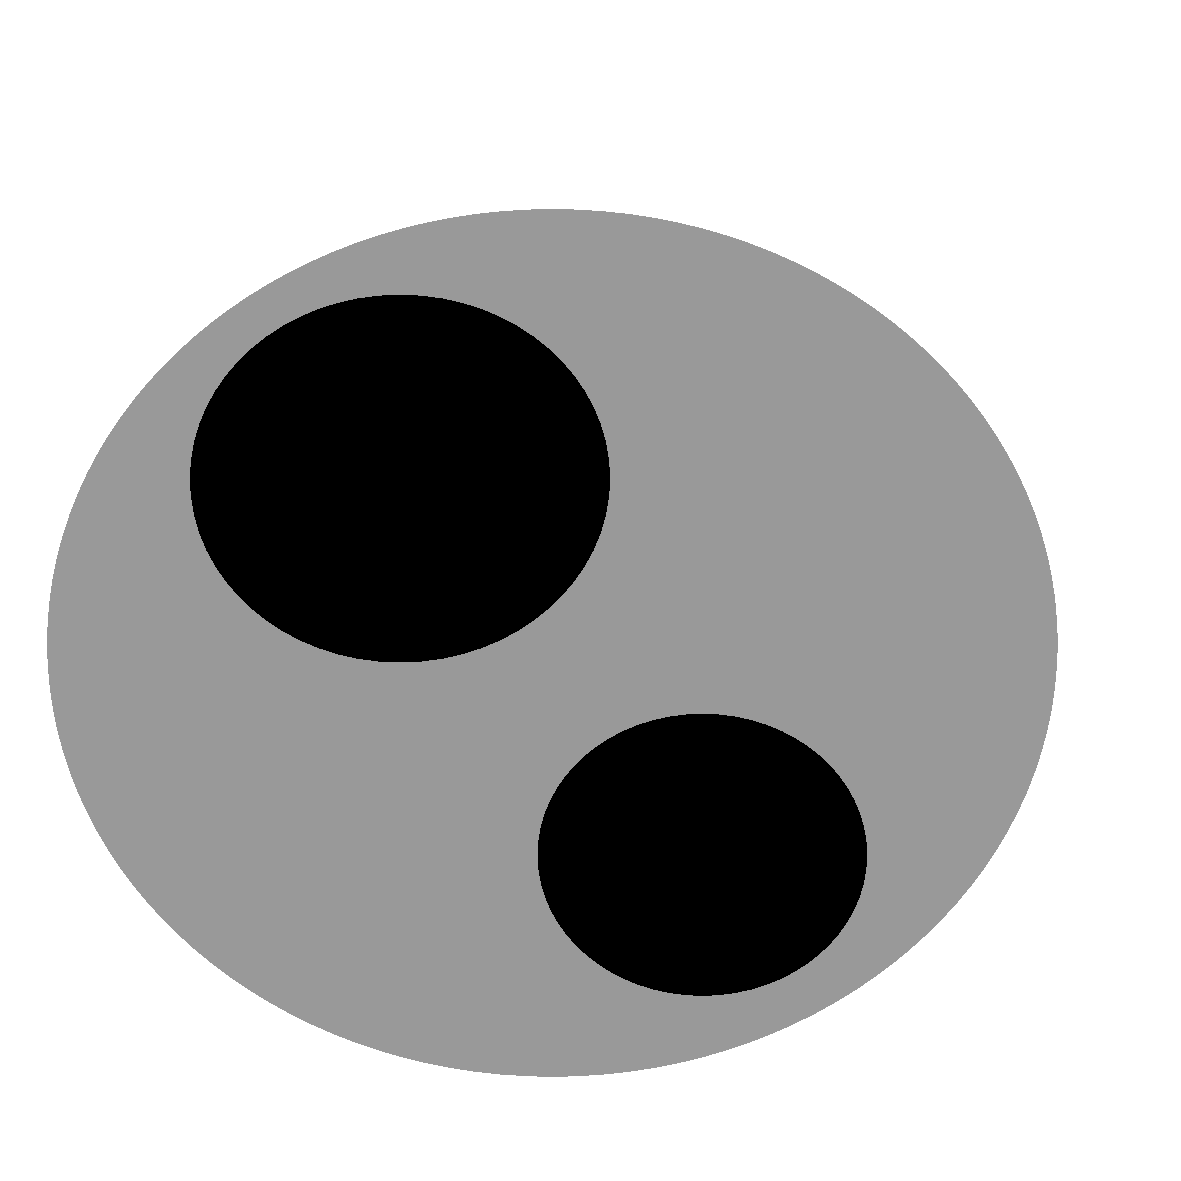
\includegraphics[width=\textwidth]{images/sur-segmentation/immerssionSim3}
		 \caption{Deux bassins versants au sein d'une même composante connexe.}
	\end{subfigure}
	\caption{Les trois cas de \modif{figure} possibles lors de la recherche de bassins versants par simulation d’\modif{inondation.}}
	\label{fig:sp:wp}
\end{figure}

Soit $A$ un ensemble et $x$ et $y$ deux éléments de $A$.  La distance géodésique entre $x$ et $y$ correspond à la \modif{longueur du plus petit chemin} reliant $x$ à $y$ et n'étant constitué que d'éléments inclus dans $A$. \modif{Soit $B$ et $C$, deux composantes connexes dont les tous les éléments sont inclus dans $A$ (c'est-à-dire que $B \subset A$ et $C \subset A$). Supposons que les éléments de $B$  et de $C$ sont parfaitement distincts. Soit $D$ le complémentaire de $B \cup C$, contenant tous les éléments de $A$ n'appartenant ni à $B$ ni à $C$. Soit $d_{i} \in D$. Soit $b_{i}$ (respectivement $c_{i}$), l'élément de $B$ le plus proche de $d_{i}$ au sens de la distance géodésique (respectivement l'élément de $C$ le plus proche de $d_{i}$ au sens de la distance géodésique). Si $b_{i}$ est plus proche de $d_{i}$ que $c_{i}$, alors $d_{i}$ appartient à la zone d'influence de $B$. Si $b_{i}$ et $c_{i}$ sont à égale distance de $d_{i}$ alors cet élément appartient au squelette des zones d'influences de $B$ et de $C$. 
} 


Ce procédé d'immersion est répété du niveau de gris le plus faible jusqu'au niveau de gris le plus élevé, afin d'obtenir une partition de l'image en superpixels. 

\section{Résultats de l'évaluation}

Les sections suivantes présentent les résultats obtenus par chacun des algorithmes évalués. Pour chaque méthode, nous avons réalisé 8 tests, en faisant varier les paramètres de manière à ce que le nombre moyen de superpixels de l'image soit respectivement proche de 500 (test 1), 700 (test 2), 900 (test 3), 1100 (test 4), 1300 (test 5), 1500 (test 6), 1700 (test 7) et 1900 (test 8) superpixels. Chaque test est effectué avec l'ensemble des images de HSID. 

 Dans les paragraphes suivants nous noterons :
\begin{itemize}
\item $N_{\mathbb{S}}$ le nombre de superpixels ;
\item $N_{V}$ : le nombre de voisins d'un \modif{superpixel} ;
\item $T$ : le temps d'exécution de la méthode ;
\item \modif{$\mathcal{F}_{FRC}$ : le score obtenu avec la mesure floue d'adhérence aux contours (équation \ref{eq:sp:FBR})}.
\end{itemize}

L'ensemble des algorithmes évalués respectant par construction la propriété \ref{prop1} (validité), nous ne nous attarderons pas sur cette dernière. La mesure $\mathcal{F}_{FRC}$ permet d'apprécier la capacité d'un algorithme à satisfaire la propriété \ref{prop2} (adhérence aux contours). Un score moyen proche de $1$ et un écart type faible, indiquent que la méthode évaluée sur-segmente correctement l'ensemble des images de HSID. 

La mise en relation de cette mesure avec le nombre de superpixels $N_{\mathbb{S}}$ conduit à une analyse du respect de la propriété \ref{prop3} (concision), en identifiant les méthodes capables d'obtenir une bonne adhérence aux contours tout en conservant un nombre peu élevé de superpixels. 

La mesure $N_{V}$ permet d'évaluer le respect de la propriété \ref{prop4} (simplicité) : il est souhaitable que le score moyen et l'écart type obtenus pour cette mesure soient aussi bas que possible.

La propriété \ref{prop5} (rapidité) est, quant à elle, évaluée à l'aide de la mesure $T$ du temps d’exécution.

Tous les algorithmes évalués ont obtenu d'excellents scores avec les mesures et les données de référence des deux évaluations précédentes \cite{achanta2012slic,stutz2015superpixel}. Le constat d'une performance moindre sur HSID, avec les mesures précédemment présentées, peut donc venir :
\begin{itemize}
\item d'une difficulté à traiter des images de grande taille, avec notamment un écart type important pour les mesures $T$ et $\mathcal{F}_{FRC}$ ;
\item d'une difficulté à traiter avec les mêmes paramètres des images de tailles \modif{différentes}, ce qu'indiqueraient des écarts types importants pour les mesures $N_{V}$, $T$ et $\mathcal{F}_{FRC}$.
\end{itemize}

Dans les deux cas, nous considérons que la méthode ne passe pas à l'échelle, puisque l'introduction d'images de taille importante se révèle problématique. 

Reste la question de l'adaptabilité d'une méthode, c'est-à-dire de sa capacité à sur-segmenter correctement des images de différentes complexités ou des images dont certaines zones sont plus complexes que d'autres. Une manière d'identifier les algorithmes possédant cette propriété consiste à s'intéresser à l'écart type de la mesure $N_{\mathbb{S}}$. Nous nous attendons à ce que ce dernier soit élevé, un faible écart type indiquant que la méthode est restée très proche du nombre moyen de superpixels recherché, sans s'adapter aux données.

L'ensemble des sur-segmentations produites par chacun des algorithmes peut être consulté en ligne\footnote{\url{http://image.ensfea.fr/hsid/}}.

\subsection{Quelques résultats généraux}

Sur l'ensemble des tests, tous les algorithmes produisent des sur-segmentations avec en moyenne $6$ voisins par superpixel, avec un écart type inférieur à $\nombre{0,2}$. En ce qui concerne la propriété de simplicité, les méthodes évaluées réalisent donc une performance équivalente.

Les figures \ref{fig:sp:fbr_nbSp} et \ref{fig:sp:time_nbSp} montrent, pour chaque algorithme, l’évolution de l'adhérence aux contours en fonction du nombre de superpixels.  Le score $\mathcal{F}_{FRC}$ donné correspond à la moyenne obtenue pour l'ensemble de HSID. Les méthodes ERS, FZ et SLIC réalisent une performance significativement meilleure que celles des algorithmes QS, CRS, BASS et WP. Dans les sections suivantes, nous aurons l'occasion d'analyser plus en détail ce que ces résultats impliquent. 


\begin{figure}[htb]
	\centering	
			\includegraphics[width=\textwidth]{images/sur-segmentation/fbr_NbSp}
		 	\caption{Évolution de l'adhérence aux contours ($\mathcal{F}_{FRC}$) en fonction du nombre de superpixels.}
		 	\label{fig:sp:fbr_nbSp}
\end{figure}

La figure \ref{fig:sp:time_nbSp} donne les temps \modif{d'exécution} moyens de chaque algorithme en fonction du nombre de superpixels.  Les deux extrêmes sont\modif{,} d'une part\modif{,} l'algorithme QS dont le temps d'exécution moyen dépasse la minute et\modif{, d'autre part,} SLIC dont la durée moyenne est de seulement $3$ secondes. Par rapport aux évaluations précédemment menées \cite{achanta2012slic, stutz2015superpixel}, nos tests font apparaître de manière nette les différences entre \modif{les algorithmes}. 

À part QS pour lequel une variation importante est visible, le nombre de superpixels produits n'influe que peu le temps d'exécution moyen. En effet, la complexité algorithmique des méthodes étudiées dépend essentiellement du nombre de pixels. 

\begin{figure}[htb]
	\centering	
			\includegraphics[width=\textwidth]{images/sur-segmentation/time_NbSp}
		 	\caption{\modif{Évolution du temps d'exécution} en fonction du nombre de superpixels.}
		 	\label{fig:sp:time_nbSp}
\end{figure}

\subsection{\modif{Méthode de Vedaldi \textit{et al.} }}

Pour évaluer la méthode QS  \cite{vedaldi2008quick}, nous avons utilisé l'implémentation de la bibliothèque VLFeat\footnote{\url{http://www.vlfeat.org/overview/quickshift.html}}. Trois paramètres doivent être spécifiés :
\begin{itemize}
\item $\omega_{c}$, qui permet de pondérer l'importance de la couleur du pixel par rapport à sa position dans l'image ;
\item $\omega_{\phi}$, qui correspond à la taille de la fenêtre d'observation gaussienne ;
\item $\omega_{d}$, qui est la distance maximale entre deux pixels $p_{i}$ et $p_{j}$ pour que $p_{j}$ soit considéré comme appartenant \modif{à l'ensemble des} plus proches voisins de $p_{i}$.
\end{itemize}

Durant les 8 tests, nous avons utilisé $\omega_{c}=\nombre{0,75}$ et $\omega_{\phi}=3$, qui correspondent aux valeurs recommandées par Stutz \textit{et al.} \cite{stutz2015superpixel} lors de leur évaluation. Le tableau \ref{tab:sp:paramQS} récapitule les valeurs utilisées pour le paramètre $\omega_{d}$.

\begin{table}[htb]
 \caption{Valeurs du paramètre $\omega_{d}$ utilisées pour évaluer la méthode QS\modif{.}}
\centering
\begin{tabular}{| l| l| l| l| l| l| l| l|  l|}
\hline
\cellcolor{gris}{Test} & 1 & 2 & 3 & 4 & 5 & 6&7 &8\\
\hline
$\cellcolor{gris}{\omega_{d}}$ & 47 & 50 &35 &30 &27 &25&20 &10\\
\hline
\end{tabular}
\label{tab:sp:paramQS}
\end{table}


L'analyse de la figure \ref{fig:sp:fbr_nbSp} montre que l'algorithme QS obtient la quatrième position en termes de respect de l'adhérence aux contours par rapport au nombre de superpixels. Le score $\mathcal{F}_{FRC}$ moyen obtenu pour chacun des tests reste significativement inférieur à celui des algorithmes ERS, FZ et SLIC.  Le tableau \ref{tab:sp:minmaxSpQS} montre que l'écart entre le nombre minimum de superpixels  et le nombre maximum de superpixels  pour chaque test est conséquent. 

\begin{table}[htb]
 \caption{Bornes de l'intervalle de variation du nombre de superpixels produits par l'algorithme QS.}
\centering
\begin{tabular}{| l| l| l| l| l| l| l| l|  l|}
\hline
\cellcolor{gris}{Test} & 1 & 2 & 3 & 4 & 5 & 6&7 &8\\
\hline
\cellcolor{gris}{min} & $12$  & $16$ &$24$ &$29$ &$38$ &$42$&$65$ &$80$\\
\hline
\cellcolor{gris}{max} &  $2045$  & $2768$ &$3596$ &$4750$ &$5803$ &$6763$&$10222$ &$13969$\\
\hline
\end{tabular}
\label{tab:sp:minmaxSpQS}
\end{table}

La figure \ref{fig:sp:qs:nbsp_pixels} permet de voir qu'il existe une corrélation entre le nombre de pixels et le nombre de superpixels produits. Si nous étudions l'ensemble des sur-segmentations produites par Quick Shift, nous constatons  que les images de grande taille produisent des sur-segmentations avec davantage de superpixels que les images de petite taille. Nous n'avons par ailleurs pas su trouver de relation simple entre $\omega_{d}$ et $N_{I}$, le nombre de pixels de l'image, qui permette d'obtenir un nombre de superpixels pertinent. Cette dépendance entre l'un des paramètres de Quick Shift et \modif{la taille} de la photographie traitée se révèle problématique lorsque les \modif{tailles} des images à sur-segmenter \modif{n'est pas connue} à l'avance, notamment lorsque ces dernières proviennent de sources diverses. C'est en particulier le cas pour le domaine d'application qui nous intéresse : celui de la segmentation interactive.

Le faible score d'adhérence aux contours s'explique par le problème évoqué précédemment :  pour les petites images, le nombre de superpixels n'est pas assez important pour permettre une sur-segmentation précise, \modif{ ce qui se répercute sur la moyenne du score $\mathcal{F}_{FRC}$.} Par ailleurs, les images contenant des objets dont les contours ne sont pas nets, notamment parce qu'ils représentent des animaux à fourrure ou les cheveux d'une personne, posent également de grosses difficultés à Quick Shift. 

\begin{figure}[htb]
	\centering	
			\includegraphics[width=\textwidth]{images/sur-segmentation/QS/spEvolution}
		 	\caption{Algorithme QS : évolution du nombre de superpixels par rapport au nombre total de pixels dans l'image.}
		 	\label{fig:sp:qs:nbsp_pixels}
\end{figure}

La figure \ref{fig:sp:exqs1} illustre ce phénomène. Elle montre les superpixels obtenus pour deux images. Dans les deux cas, le paramètre $\omega_{d}$ vaut $47$. Pour la figure \ref{fig:sp:exqs1}a, qui correspond à une photographie de $732 \times 509$ pixels, nous obtenons $57$ superpixels. Au contraire, la photographie de la figure \modif{\ref{fig:sp:exqs1}b}, qui contient $3648 \times 2736$ pixels, est sur-segmentée en $1204$ superpixels. Enfin, le temps d'exécution moyen, même s'il décroît à mesure que le nombre de superpixels augmente, se classe parmi les plus élevés, certaines images nécessitant plusieurs minutes pour être sur-segmentées.

\modif{Ces résultats nous conduisent} à conclure que, malgré ses bonnes performances dans les études précédentes, la méthode Quick Shift ne passe pas à l'échelle et échoue à sur-segmenter convenablement HSID.

 
\begin{figure}[htb]
	\centering
	 \begin{subfigure}[t]{0.6\textwidth}	
			\includegraphics[width=\textwidth]{images/sur-segmentation/QS/Ex1-img-100}
		 	\caption{Superpixels obtenus pour l'image img-100 de HSID. Cette image comporte $732 \times 509$ pixels.}
	\end{subfigure}
 \\
	 \begin{subfigure}[t]{0.6\textwidth}	
			\includegraphics[width=\textwidth]{images/sur-segmentation/QS/Ex2-img-041}
		 	\caption{Superpixels obtenus pour l'image img-041 de HSID. Cette image comporte $3648 \times 2736$ pixels.}
	\end{subfigure}
	\caption{Algorithme Quick Shift : exemples de sur-segmentations obtenues lors du test 1, pour des images de tailles différentes. }
	\label{fig:sp:exqs1}
\end{figure}

 \subsection{Algorithme de Felzenszwalb \textit{et al.}}
 
Afin d'évaluer l'algorithme de Felzenszwalb \textit{et al.} \cite{felzenszwalb2004efficient}, nous avons utilisé l'implémentation mise à disposition par les auteurs. Elle nécessite de fixer trois paramètres : 
 \begin{itemize}
 \item  $\omega_{k}$ qui pondère l'influence des différences internes à une composante connexe, par rapport aux différences entre deux composantes connexes ;
 \item $\omega_{\sigma}$, le paramètre du filtre gaussien qui, lors d'un prétraitement, permet de réduire le bruit au sein des images ;
 \item $\omega_{min}$, la taille minimale des superpixels. 
 \end{itemize}
 
 Lors de l'ensemble de nos tests, nous avons utilisé $\omega_{k} = 24$ et $\omega_{\sigma}=\nombre{0,5}$. Ces deux paramètres découlent de tests effectués sur deux autres ensembles d'images : celles mises à disposition par McGuinness \textit{et al.} \cite{mcguinness2010comparative} et celles de Santner \textit{et al.} \cite{santner2010interactive}, les paramètres trouvés par Stutz \textit{et al.} ne se révélant pas pertinents pour HSID. Pour le paramètre $\omega_{min}$, nous avons utilisé les valeurs données dans le tableau \ref{tab:sp:paramFZ}. 

\begin{table}[htb]
 \caption{Valeurs du paramètre $\omega_{min}$ utilisées pour l'algorithme de Felzenszwalb \textit{et al}. La variable $N_{I}$ correspond au nombre de pixels de l'image. }
\centering
\begin{tabular}{| l| l| l| l| l| l| l| l|  l|}
\hline
\cellcolor{gris}{Test} & 1 & 2 & 3 & 4 & 5 & 6&7 &8\\
\hline
$\cellcolor{gris}{\omega_{min}}$ & $ N_{I}/2500$ &  $ N_{I}/3500$  & $ N_{I}/4500$  & $ N_{I}/5500$  & $ N_{I}/6500$  & $N_{I}/7500$ &  $ N_{I}/7500$ & $ N_{I}/8500$ \\
\hline
\end{tabular}
\label{tab:sp:paramFZ}
\end{table}

Les résultats obtenus par l'algorithme FZ \modif{montrent} qu'il permet de garantir une bonne adhérence aux contours. Pour l'ensemble des tests, nous constatons un écart type élevé pour la mesure $N_{\mathbb{S}}$, égal à environ un cinquième de la valeur de la moyenne. Mis en relation avec les bons scores d'adhérence aux contours, ce résultat révèle que l'algorithme de Felzenszwalb \textit{et al.} bénéficie d'une bonne adaptabilité, ce que confirme l'étude des sur-segmentations produites et ce qu'illustrent les deux exemples de la figure \ref{fig:sp:exfz1}.
 
 L'un des reproches fréquemment adressés à la méthode de Felzenszwalb \textit{et al.} concerne l'aspect des superpixels qu'elle produit, avec des bordures souvent très sinueuses, donnant un aspect moins visuellement plaisant que des algorithmes tels que SLIC ou celui de Liu \textit{et al.}. Les superpixels de la figure \ref{fig:sp:exfz1} sont effectivement assez irréguliers. De plus, la topologie des deux sur-segmentations présente des aspects surprenants tels qu'un superpixel inclus à l'intérieur d'un autre superpixel de grande taille. La  moyenne et l'écart type de la mesure $N_{V}$ révèlent toutefois qu'en termes de nombre de superpixels voisins, l'algorithme de Felzenszwalb produit des résultats similaires à ceux des autres algorithmes évalués, avec un score de $6$, ce qui reste inférieur au nombre de voisins \modif{d'un} pixel si nous considérons le 8-voisinage.

Le  temps d'exécution moyen de l'algorithme gravite autour d'une dizaine de secondes et tend à diminuer légèrement lorsque le nombre de superpixels augmente. 

L'ensemble de ces résultats nous conduit à conclure que l'algorithme de Felzenszwalb \textit{et al.} passe correctement à l'échelle, en réussissant à sur-segmenter les images de HSID de manière à conserver une bonne adhérence aux contours, sans que le nombre de superpixels n'explose. 
 
 \begin{figure}[htb]
	\centering
	 \begin{subfigure}[t]{0.55\textwidth}	
			\includegraphics[height=0.4\textheight]{images/sur-segmentation/FZ/EX1-img-086}
		 	\caption{Superpixels obtenus pour l'image img-086 de HSID.}
	\end{subfigure}
	~ 
	 \begin{subfigure}[t]{0.4\textwidth}	
			\includegraphics[height=0.4\textheight]{images/sur-segmentation/FZ/EX2-img-028}
		 	\caption{Superpixels obtenus pour l'image img-028 de HSID.}
	\end{subfigure}
	\caption{Algorithme de Felzenszwalb \textit{et al.} : exemples de sur-segmentations obtenues lors du test 8. }
	\label{fig:sp:exfz1}
\end{figure}
 
 \subsection{Algorithme de Liu \textit{et al.}}
 Pour évaluer l'algorithme de Liu \textit{et al.} \cite{liu2011entropy}, nous avons utilisé l'implémentation fournie par les auteurs ainsi que les paramètres recommandés par Stutz \textit{et al.} \cite{stutz2015superpixel}. Les paramètres à spécifier sont les suivants :
 \begin{itemize}
 \item $\omega_{\sigma}$, qui correspond à l'écart type d'une fonction gaussienne utilisée pour calculer la mesure de similarité entre deux pixels à partir de la valeur absolue de la différence entre les niveaux de gris des pixels ;
 \item $\omega_{\lambda}$, qui permet de pondérer l'influence entre les termes $\mathcal{F}_{R}$ et $\mathcal{F}_{E}$ de la \modif{fonction de coût} ;
 \item $\omega_{N_{\mathbb{S}}}$, le nombre de superpixels souhaité. 
 \end{itemize}
 

 Durant tous les tests, nous avons considéré des pixels voisins au sens du 8-voisinage, $\omega_{\sigma}=\nombre{0,21}$ et $\omega_{\lambda}=\nombre{0,5}$. Pour le paramètre $\omega_{N_{\mathbb{S}}}$, nous avons utilisé les valeurs présentées dans le tableau \ref{tab:sp:paramERS}.
 \begin{table}[htb]
 \caption{Valeurs du paramètre $\omega_{N_{\mathbb{S}}}$ utilisées pour évaluer l'algorithme de Liu \textit{et al.}}
\centering
\begin{tabular}{| l| l| l| l| l| l| l| l|  l|}
\hline
\cellcolor{gris}{Test} & 1 & 2 & 3 & 4 & 5 & 6&7 &8\\
\hline
$\cellcolor{gris}{\omega_{N_{\mathbb{S}}}}$ & 500 & 700 & 900 &1100 &1300 &1500&1700 &1900\\
\hline
\end{tabular}
\label{tab:sp:paramERS}
\end{table}

 
De toutes les méthodes évaluées, celle de Liu \textit{et al.} obtient la meilleure adhérence aux contours avec un minimum de superpixels. Cette très bonne performance doit cependant être nuancée par  des temps d'exécution importants (plus d'une minute pour certaines images) et l'absence complète d'adaptabilité, le nombre de superpixels étant un paramètre fixé par l'utilisateur de la méthode. Le premier de ces inconvénient limite l'utilisation de la méthode à des applications où les temps de calcul ne sont pas trop critiques. Ce n'est malheureusement pas le cas du domaine applicatif qui nous intéresse, celui de la segmentation interactive. Quant à l'absence d'adaptabilité, elle se traduit par deux désavantages : d'une part, certaines images relativement simples sont sur-segmentées en davantage de superpixels que nécessaire. D'autre part, pour les images les plus complexes, même avec $1900$ superpixels, certains détails sont perdus.
 
  \begin{figure}[htb]
	\centering
	 \begin{subfigure}[t]{0.45\textwidth}	
			\includegraphics[width=\textwidth]{images/sur-segmentation/ERS/EX1-img-042}
		 	\caption{Superpixels obtenus pour l'image img-042 de HSID.}
	\end{subfigure}
 ~
	 \begin{subfigure}[t]{0.45\textwidth}	
			\includegraphics[width=\textwidth]{images/sur-segmentation/ERS/EX2-img-058}
		 	\caption{Superpixels obtenus pour l'image img-058 de HSID.}
	\end{subfigure}
	\caption{Algorithme de Liu \textit{et al.} : exemples de sur-segmentations obtenues lors du test 6. }
	\label{fig:sp:exers1}
\end{figure}
 

 Les deux exemples présentés sur la figure \ref{fig:sp:exers1} soulignent ce paradoxe : si les sur-segmentations produites suivent parfaitement les contours des objets, malgré le fait que les photographies présentent de nombreuses difficultés (objets voisins de couleurs similaires, bruit, ombre, etc.), elles comprennent de nombreux petits superpixels qui pourraient être fusionnés. 
 
 \subsection{\modif{Méthode  d'Achanta \textit{et al.}}}
\label{subsec:sp:res-slic}
 
 Afin d'évaluer l'algorithme SLIC \cite{achanta2012slic}, nous avons utilisé l'implémentation mise à disposition par Achanta \textit{et al.} Cette dernière requiert de spécifier : 
 \begin{itemize}
 \item \modif{$\omega_{C}$}, le paramètre de compacité pondérant l'influence de la localisation d'un pixel par rapport à sa couleur ; , le nombre approximatif de superpixels souhaité, qui permet de produire la sur-segment
 \item $\omega_{N_{\mathbb{S}}}$, le nombre approximatif de superpixels souhaité, qui permet de produire la sur-segmentation de départ, sous forme de grille.
 \end{itemize}
 
Suivant les recommandations d'Achanta \textit{et al.} \cite{achanta2012slic} et celles de Stutz \textit{et al.} \cite{stutz2015superpixel}, nous avons utilisé \modif{$\omega_{C} = 10$} pour l'ensemble de nos tests. Les valeurs du paramètre  $\omega_{N_{\mathbb{S}}}$ sont données dans le tableau \ref{tab:sp:paramSLIC}.

 \begin{table}[htb]
 \caption{Valeurs du paramètre $\omega_{N_{\mathbb{S}}}$ utilisées pour évaluer l'algorithme SLIC.}
\centering
\begin{tabular}{| l| l| l| l| l| l| l| l|  l|}
\hline
\cellcolor{gris}{Test} & 1 & 2 & 3 & 4 & 5 & 6&7 &8\\
\hline
$\cellcolor{gris}{\omega_{N_{\mathbb{S}}}}$ & 500 & 700 & 900 &1100 &1300 &1500&1700 &1900\\
\hline
\end{tabular}
\label{tab:sp:paramSLIC}
\end{table}


 SLIC nécessite davantage de superpixels que les algorithmes de Felzenszwalb \textit{et al.} \cite{felzenszwalb2004efficient} et de Liu \textit{et al.} \cite{liu2011entropy} pour obtenir une adhérence aux contours semblable, avec un score $\mathcal{F}_{FRC}$ égal à $\nombre{0,59}$ atteint avec \modif{quasiment} $1900$ superpixels, tandis que les deux méthodes précédemment citées réalisent la même performance avec respectivement $1600$ et $1300$ superpixels. En termes d'adaptabilité, l'algorithme de Felzenszwalb se révèle également légèrement meilleur que SLIC \modif{: adapter le nombre de superpixels au niveau de détail de l'image reste à la charge de l'utilisateur.} Le principal atout de SLIC reste cependant ses temps d'exécution, largement \modif{inférieurs} à ceux des autres méthodes, avec un temps moyen de $3$ secondes.

 
  \begin{figure}[htb]
	\centering
	 \begin{subfigure}[t]{0.45\textwidth}	
			\includegraphics[width=\textwidth]{images/sur-segmentation/SLIC/EX1-img-046}
		 	\caption{Superpixels obtenus pour l'image img-046 de HSID.}
	\end{subfigure}
 ~
	 \begin{subfigure}[t]{0.45\textwidth}	
			\includegraphics[width=\textwidth]{images/sur-segmentation/SLIC/EX2-img-052}
		 	\caption{Superpixels obtenus pour l'image img-052 de HSID.}
	\end{subfigure}
	\caption{Algorithme SLIC: exemples de sur-segmentations \modif{obtenues lors du test 8}.}
	\label{fig:sp:exslic1}
\end{figure}


  \subsection{Algorithme de Rubio \textit{et al.}}
Afin de tester l'algorithme de Rubio \textit{et al.} \cite{rubio2016bass}, nous avons utilisé l'implémentation mise à disposition par ses auteurs. Le seul paramètre de cette méthode est $\omega_{N_{\mathbb{S}}}$, le nombre initial de superpixels, pour lequel nous avons utilisé les valeurs du tableau \ref{tab:sp:BASSParam}.

\begin{table}[htb]
\caption{Valeurs du paramètre $\omega_{N_{\mathbb{S}}}$ utilisées lors des tests effectués avec la méthode de Rubio \textit{et al.}}
\centering
\begin{tabular}{|l|l|l|l|l|l|l|l|l|}
\hline
\cellcolor{gris}{\modif{Test} }& 1 & 2 & 3 &4 & 5&6 &7 &8 \\
\hline
$\cellcolor{gris}{\omega_{N_{\mathbb{S}}}}$&700&1100&1500&1900&2300&2700&3100&3500 \\
\hline
\end{tabular}
\label{tab:sp:BASSParam}
\end{table}

L'analyse des résultats de l'algorithme de Rubio \textit{et al.}, permet de mettre en exergue l'importance de la mise à disposition de HSID. Dans l'article \cite{rubio2016bass} où ils décrivent leur algorithme, Rubio \textit{et al.} le comparent à quelques méthodes de l'état de l'art, dont SLIC, sur sept \modif{ensembles de données de référence différents} \modif{\cite{kolesnikov2014closed,liu2011learning,MartinFTM01,yamaguchi2012parsing,yan2014hierarchical}}, totalisant plusieurs milliers d'images comprenant des difficultés très variées mais dont les \modif{tailles} sont toujours \modif{proches} : quelques centaines de pixels en largeur comme en hauteur, pour un nombre total de pixels $N_{I} \backsimeq 15000$. Une autre propriété commune à l'ensemble des photographies est qu'elles contiennent en majorité des objets bénéficiant d'un bon contraste avec le fond. Les résultats obtenus par Rubio \textit{et al.} montrent que leur méthode obtient de meilleurs résultats que SLIC, avec un nombre \modif{inférieur de superpixels.} 

Nos tests avec HSID ne permettent pas d'aboutir à la même conclusion :  le score d'adhérence aux contours de la méthode de Rubio \textit{et al.} est largement en dessous de celui de SLIC. Les deux exemples donnés sur la figure \ref{fig:sp:exbass1} montrent que les mécanismes qui garantissent à l'algorithme de Rubio \textit{et al.} une bonne adaptabilité sont responsables des erreurs importantes commises, là où la présence des contours des objets est difficilement perceptible.

Par ailleurs, les modifications introduites par Rubio \textit{et al.} afin d'obtenir une méthode avec une meilleure adaptabilité se paient par une augmentation considérable des temps d’exécution, avec une moyenne d'environ $40$ secondes, soit plus de dix fois le temps d'exécution moyen de SLIC. Notons que les algorithmes de Felzenszwalb \textit{et al.} \cite{felzenszwalb2004efficient} et de Liu \textit{et al.} \cite{liu2011entropy} (avec lesquels Rubio \textit{et al.} ne comparent pas leur méthode), obtiennent eux aussi une bien meilleure adhérence aux contours, avec des temps d'exécution inférieurs.
 
 
   \begin{figure}[htb]
	\centering
	 \begin{subfigure}[t]{0.45\textwidth}	
			\includegraphics[width=\textwidth]{images/sur-segmentation/BASS/EX1-img-012}
		 	\caption{Superpixels obtenus pour l'image img-012 de HSID.}
	\end{subfigure}
 ~
	 \begin{subfigure}[t]{0.45\textwidth}	
			\includegraphics[width=\textwidth]{images/sur-segmentation/BASS/EX2-img-040}
		 	\caption{Superpixels obtenus pour l'image img-040 de HSID.}
	\end{subfigure}
	\caption{Algorithme de Rubio \textit{et al.}: exemples de sur-segmentations \modif{obtenues lors du test~1}.}
	\label{fig:sp:exbass1}
 \end{figure}

 \subsection{Algorithme de Conrad \textit{et al.}}
 
 Afin de tester l'algorithme de Conrad \textit{et al.} \cite{conrad2013contour}\modif{,} nous avons utilisé l'implémentation que les auteurs ont mise à disposition. Les paramètres de cette implémentation sont les suivants :
 \begin{itemize}
 \item $\omega_{R}$, le paramètre permettant de pondérer l'influence du terme de régularisation de la fonction à maximiser ;
 \item $\omega_{4V}$, le paramètre permettant de pondérer la pénalité prise en compte lorsque l'un des quatre voisins d'un pixel n'appartient pas au même superpixel ;
 \item $\omega_{D}$, le paramètre permettant de pondérer la pénalité prise en compte lorsque l'un des voisins diagonaux d'un pixel n'appartient pas au même superpixel ;
 \item $\omega_{Iter}$, le nombre d'itérations de l'algorithme ;
 \item $\omega_{N_{\mathbb{S}}}$, le nombre initial de superpixels.
 \end{itemize}
 Pour l'ensemble de nos tests, nous avons utilisé $\omega_{R}=\nombre{0,045}$, $\omega_{4V}=\nombre{0,3}$, $\omega_{D}=\nombre{0,21}$ et $\omega_{Iter}=3$, valeurs recommandées par Stutz \textit{et al.} \cite{stutz2015superpixel}. Pour le paramètre $\omega_{N_{\mathbb{S}}}$ nous avons utilisé les valeurs données dans le tableau \ref{tab:sp:CRSParam}.
  \begin{table}[htb]
\caption{Valeurs du paramètre $\omega_{N_{\mathbb{S}}}$ utilisées lors des tests effectués avec la méthode de Conrad \textit{et al.}}
\centering
\begin{tabular}{|l|l|l|l|l|l|l|l|l|}
\hline
\cellcolor{gris}{\modif{Test}  }& 1 & 2 & 3 &4 & 5&6 &7 &8 \\
\hline
$\cellcolor{gris}{\omega_{N_{\mathbb{S}}}}$&500&700&900&1100&1300&1500&1700&1900 \\
\hline
\end{tabular}
\label{tab:sp:CRSParam}
\end{table}

L'analyse des résultats obtenus par CRS  \cite{conrad2013contour}  amène au constat que la méthode ne parvient pas à sur-segmenter correctement HSID, avec des scores pour la mesure $\mathcal{F}_{FRC}$ faibles, y compris pour un nombre élevé de superpixels. Une étude visuelle des sur-segmentations produites montre que si les images de \modif{taille} modeste (quelques milliers de pixels) sont sur-segmentées correctement, la méthode de Conrad \textit{et al.} échoue à produire des superpixels corrects pour les images de grande taille (plusieurs millions de pixels). Une illustration est donnée sur la figure \ref{fig:sp:excrs1}. 
  
Le fait que l'algorithme de Conrad \textit{et al.} ne passe pas à l'échelle s'explique par sa trop grande dépendance vis-à-vis de la sur-segmentation initiale, une grille régulière de $\omega_{N_{\mathbb{S}}}$ cases. Pour les images de grande taille contenues dans HSID,  cette sur-segmentation initiale correspond à une erreur importante par rapport à la sur-segmentation souhaitée. En ne modifiant, à chaque itération, que les pixels au niveau des contours, la convergence vers un résultat acceptable devient très lente. Il n'est par ailleurs  pas assuré qu'en augmentant le nombre d'itérations, un meilleur score moyen pour la mesure $\mathcal{F}_{FRC}$ soit atteint : les caractéristiques (moyenne et variance de la couleur des pixels) initiales calculées étant elles aussi entachées d'erreurs conséquentes. Lors de tests complémentaires, nous avons multiplié par $100$ le nombre d'itérations, sans constater d'amélioration notable de l'adhérence aux contours. Les temps d'exécution, quant à eux, dépassaient les trentes minutes par image. 


    \begin{figure}[htb]
	\centering
	 \begin{subfigure}[t]{0.45\textwidth}	
			\includegraphics[width=\textwidth]{images/sur-segmentation/CRS/EX1-img-003}
		 	\caption{Superpixels obtenus pour l'image img-003 de HSID, avec $2121 \times 2816$ pixels.}
	\end{subfigure}
	~
	 \begin{subfigure}[t]{0.45\textwidth}	
			\includegraphics[width=\textwidth]{images/sur-segmentation/CRS/EX1-img-003-ext1}
		 	\caption{Superpixels obtenus pour l'image img-003 de HSID (zoom).}
	\end{subfigure}
 \\
	 \begin{subfigure}[t]{0.45\textwidth}	
			\includegraphics[width=\textwidth]{images/sur-segmentation/CRS/EX2-img-095}
		 	\caption{Superpixels obtenus pour l'image img-095 de HSID, avec $ 800 \times 535$ \modif{pixels}.}
	\end{subfigure}
	~
	 \begin{subfigure}[t]{0.45\textwidth}	
			\includegraphics[width=\textwidth]{images/sur-segmentation/CRS/EX2-img-095-ext1}
		 	\caption{Superpixels obtenus pour l'image img-0095 de HSID (zoom). }
	\end{subfigure}
	\caption{Algorithme de Conrad \textit{et al.}: exemples de sur-segmentations obtenues lors du test 8.}
	\label{fig:sp:excrs1}
\end{figure}

 \subsection{Algorithme de Machairas \textit{et al.}}
 Afin d'évaluer la méthode Machairas \textit{et al.} \cite{machairas2015waterpixels}, nous avons utilisé l'exécutable\footnote{Nous n'avons malheureusement pas pu avoir accès au code source.} que ses auteurs ont mis à disposition. Ce dernier nécessite deux paramètres :
 \begin{itemize}
 \item $\omega_{R}$, un paramètre de régularisation, permettant d'obtenir des superpixels dont les contours sont plus ou moins réguliers ;
 \item $\omega_{N_{\mathbb{S}}}$, le nombre approximatif de superpixels souhaité.
 \end{itemize}
 
 Durant l'ensemble de nos tests, nous avons utilisé $\omega_{R}=8$, qui correspond à la valeur recommandée par Machairas \textit{et al.} \modif{et} qui \modif{donne} les meilleurs résultats sur HSID. Les valeurs du paramètre $\omega_{N_{\mathbb{S}}}$ sont \modif{récapitulées} dans le tableau \ref{tab:sp:WPParam}.
 
 \begin{table}[htb]
\caption{Valeurs du paramètre $\omega_{N_{\mathbb{S}}}$ utilisées lors des tests effectués avec la méthode de Machairas \textit{et al.}}
\centering
\begin{tabular}{|l|l|l|l|l|l|l|l|l|}
\hline
\cellcolor{gris}{\modif{Test}  }& 1 & 2 & 3 &4 & 5&6 &7 &8 \\
\hline
$\cellcolor{gris}{\omega_{N_{\mathbb{S}}}}$&500&700&900&1100&1300&1500&1700&1900 \\
\hline
\end{tabular}
\label{tab:sp:WPParam}
\end{table}

 Contrairement aux autres algorithmes, celui de Machairas \textit{et al.} échoue à produire un résultat pour les images \emph{img-012}, \emph{img-066} et \emph{img-072} de HSID. Ne disposant pas du code source, nous n'avons pas pu déterminer la cause de ce comportement. Nos tests ont donc été réalisés sur une version tronquée \modif{de HSID}, ne contenant pas ces trois images.
 

Les résultats obtenus par l'algorithme de Machairas \textit{et al.} sont un nouvel exemple d'une méthode obtenant de bons résultats \modif{sur les} données de référence BSD, mais échouant à sur-segmenter correctement les images de HSID. Ainsi, malgré un nombre important de superpixels (supérieur à 2000), l'adhérence aux contours reste très inférieure à celle obtenue avec des algorithmes tels que celui de Liu \cite{liu2011entropy}, de Felzenszwalb \cite{felzenszwalb2004efficient} ou la méthode SLIC \cite{achanta2012slic}. Les temps d’exécution sont quant à eux assez élevés, une vingtaine de secondes en moyenne. 
 
 L'analyse visuelle des résultats obtenus montre d'importantes disparités entre les \modif{sur-seg\-men\-ta\-tions} des images de grande taille et celles de petite taille. Ainsi, comme l'illustre la figure \ref{fig:sp:exwp1}, alors que les superpixels obtenus pour des images de \modif{grande taille} (figures \ref{fig:sp:exwp1}a et \ref{fig:sp:exwp1}b) sont souvent erronés, ceux des photographies de quelques milliers de pixels (\modif{voir les figures} \ref{fig:sp:exwp1}c et \ref{fig:sp:exwp1}d) garantissent une adhérence aux contours bien meilleure.
 

\begin{figure}[b]
	\centering
	 \begin{subfigure}[t]{0.45\textwidth}	
			\includegraphics[width=\textwidth]{images/sur-segmentation/WP/EX1-img-020}
		 	\caption{Superpixels obtenus pour l'image img-020 de HSID.}
	\end{subfigure}
	~
	 \begin{subfigure}[t]{0.45\textwidth}	
			\includegraphics[width=\textwidth]{images/sur-segmentation/WP/EX1-img-020-Zoom}
		 	\caption{Superpixels obtenus pour l'image img-020 de HSID (zoom).}
	\end{subfigure}
	\\
	 \begin{subfigure}[t]{0.45\textwidth}	
			\includegraphics[width=\textwidth]{images/sur-segmentation/WP/EX2-img-099}
		 	\caption{Superpixels obtenus pour l'image img-099 de HSID.}
	\end{subfigure}
	~
	 \begin{subfigure}[t]{0.45\textwidth}	
			\includegraphics[width=\textwidth]{images/sur-segmentation/WP/EX2-img-099-Zoom}
		 	\caption{Superpixels obtenus pour l'image img-099 de HSID (zoom).}
	\end{subfigure}
	\caption{Algorithme de Machairas \textit{et al.}: exemples de sur-segmentations obtenues lors du test 8.}
	\label{fig:sp:exwp1}
\end{figure}

\subsection{Choix d'une méthode de sur-segmentation}

L'évaluation conduite à partir des images \modif{de HSID} montre que seulement trois méthodes --~SLIC \cite{achanta2012slic}, l'algorithme de Felzenszwalb \textit{et al.} \cite{felzenszwalb2004efficient} et celui de Liu \textit{et al.} \cite{liu2011entropy} -- sur-segmentent correctement un ensemble d'images de taille variable, dont certaines contiennent plusieurs millions de pixels. Dans le domaine applicatif qui nous concerne, la méthode de sur-segmentation choisie doit être intégrée au sein d'une méthode de segmentation interactive, capable de produire un résultat en quelques secondes. À ce titre, malgré son excellente adhérence aux contours, l'algorithme de Liu \textit{et al.} \cite{liu2011entropy} ne peut être utilisé en raison de ses temps d'exécution élevés. 

Si l'algorithme de Felzenszwalb \textit{et al.} \cite{felzenszwalb2004efficient} bénéficie d'une meilleure adaptabilité que SLIC, il reste néanmoins significativement plus lent. Par ailleurs, les superpixels produits par cet algorithme peuvent avoir une aire importante, entraînant des erreurs \modif{conséquentes} lorsque la bordure entre deux objets est difficile à détecter. L'une des contraintes fortes de l'algorithme de segmentation interactive que nous proposons réside dans le fait qu'une erreur commise lors de l'étape de sur-segmentation ne peut être corrigée par la suite, quels que soient les germes données par l'utilisateur. Même si ce type d'erreur demeure marginal, lorsqu'il survient, il place l'utilisateur dans l'impossibilité d'aboutir à un résultat acceptable\modif{. \textit{A contrario}}, les faibles temps d'exécution de SLIC permettent de compenser le fait qu'un nombre plus important de superpixels doivent être produits pour sur-segmenter correctement l'image. Par ailleurs, ces superpixels étant de petite taille, lorsqu'une erreur est commise, son impact sur le résultat final reste faible.

Toutes ces raisons nous ont conduit à privilégier l'utilisation de SLIC au sein de la méthode de segmentation interactive que nous proposons.

\section{Conclusion}

Si l'objectif du protocole d'évaluation présenté dans ce chapitre concernait le choix d'une méthode de sur-segmentation pertinente dans le cadre \modif{d'un} domaine d'application particulier\modif{,} celui de la segmentation interactive\modif{, }l'analyse des résultats obtenus met également en évidence l'apport de HSID. 

En particulier, nous notons que le fait que HSID contienne des images dont \modif{la taille va} de quelques milliers à plusieurs millions de pixels permet :
\begin{itemize}
\item d'identifier des méthodes dont les paramètres dépendent de la taille de la photographie à sur-segmenter, à l'instar des conclusions obtenues avec Quick Shift \cite{vedaldi2008quick} ;
\item de constater que certains algorithmes, comme celui de Conrad \textit{et al.} \cite{conrad2013contour}, ont été optimisés pour de petites images et n'arrivent pas à sur-segmenter correctement des images de \modif{taille} bien \modif{supérieure} ;
\item de repérer des difficultés de passage à l'échelle, notamment vis-à-vis des temps d'exécution, par exemple avec l'algorithme de Liu \textit{et al.} \cite{liu2011entropy} dont l'écart avec des méthodes telles que SLIC \modif{\cite{achanta2012slic}} ou celle de Felzenszwalb \textit{et al.} \modif{\cite{felzenszwalb2004efficient}} devient nettement plus perceptible.
\end{itemize}

Par ailleurs, les résultats obtenus par la méthode de Rubio \textit{et al.} \cite{rubio2016bass} ou par celle de Machairas \textit{et al.} \cite{machairas2015waterpixels} montrent, qu'au delà des aspects liés à la taille des photographies, les images de HSID présentent des difficultés plus marquées que dans d'autres ensembles de données de référence.


 